% !TEX root = ../main.tex
\chapter{基于自注意力机制的通用大规模检索}
由于其检索的速度以及较低的内存开销, 深度哈希在大规模图像检索领域获得了广泛的关注。直到本章的算法提出前, 这个领域的所有的深度哈希模型都是基于卷积神经网络而设计, 例如, \textbf{ResNet}~\cite{he2016deep}, \textbf{AlexNet}等。在本章中, 受最近Vision Transformer架构的启发, 我们设计了第一个完全基于Vision Transformer的深度哈希架构来进行大规模的图像检索。具体来说, 我们的架构包含两个基本的模块: (1) 基于Vision Transformer (ViT), 我们设计了一个孪生Vison Transformer的主干架构来进行特征提取。为了学习细粒度的特征, 我们设计了一个双流特征学习的Transformer块来同时学习局部和全局的特征。(2)同时, 我们采取一个基于动态创建的相似度矩阵作为监督标签设计的贝叶斯学习框架来学习相似度保持的紧凑的二进制哈希编码。整个框架是通过一种端到端的方法同一训练。据我们所知, 本章提出的深度哈希框架是第一个完全不基于卷积神经网络的深度哈希学习框架。本章的算法在三个被广泛研究的标准数据集上进行全方面的测试, 数据集包括:~\textbf{CIFAR-10},~\textbf{NUSWIDE},~和~\textbf{IMAGENET}。数据结果证实了我们的方法和现阶段的先进的深度哈希算法比较具有极高的性能的优越性。在三个数据集上, 我们比较第二优越的算法分别获得了 $8.2\%$, $2.6 \%$和$12.7\%$的性能增长。

\section{引言}
近些年来, 由于互联网技术的普及, 以及计算机技术, 便携摄像的进步, 传感器技术, 云计算以及各种社交网络的兴起, 由无数终端用户生成的视频和图片数据以爆炸性的速度增长。如何对海量的数据进行检索是利用数据进行其他大规模商业应用的基石, 因此准确和高效进行数据检索的研究开始受到学术界和工业界研究人员的大规模的关注。在这些技术研究中, 大规模图像检索由于其广泛的工业界应用, 如推荐系统, 搜索引擎, 遥感检索系统等, 受到了日益增长的关注。 在所有解决这一具有挑战性的任务的方法中\cite{fu2017fast, ge2013optimized, jegou2010product, malkov2018efficient}, 基于二进制码的哈希方法取得了令人瞩目的成果。基于哈希的方法通过学习一个哈希函数, 将高维像素空间中的图片映射到低维的二进制汉明空间中, 其中在低维度的汉明空间的图片对应的哈希码需要保存原图片之间的视觉相似性。过去的年, 一大批的基于哈希的方法被提出。 根据它们提取特征的方法, 我们可以将其简单的分成两个类别: (1) 基于手工特征提取的方法 (2) 基于深度学习的方法。\par

\begin{figure}[!htp]
    \centering
    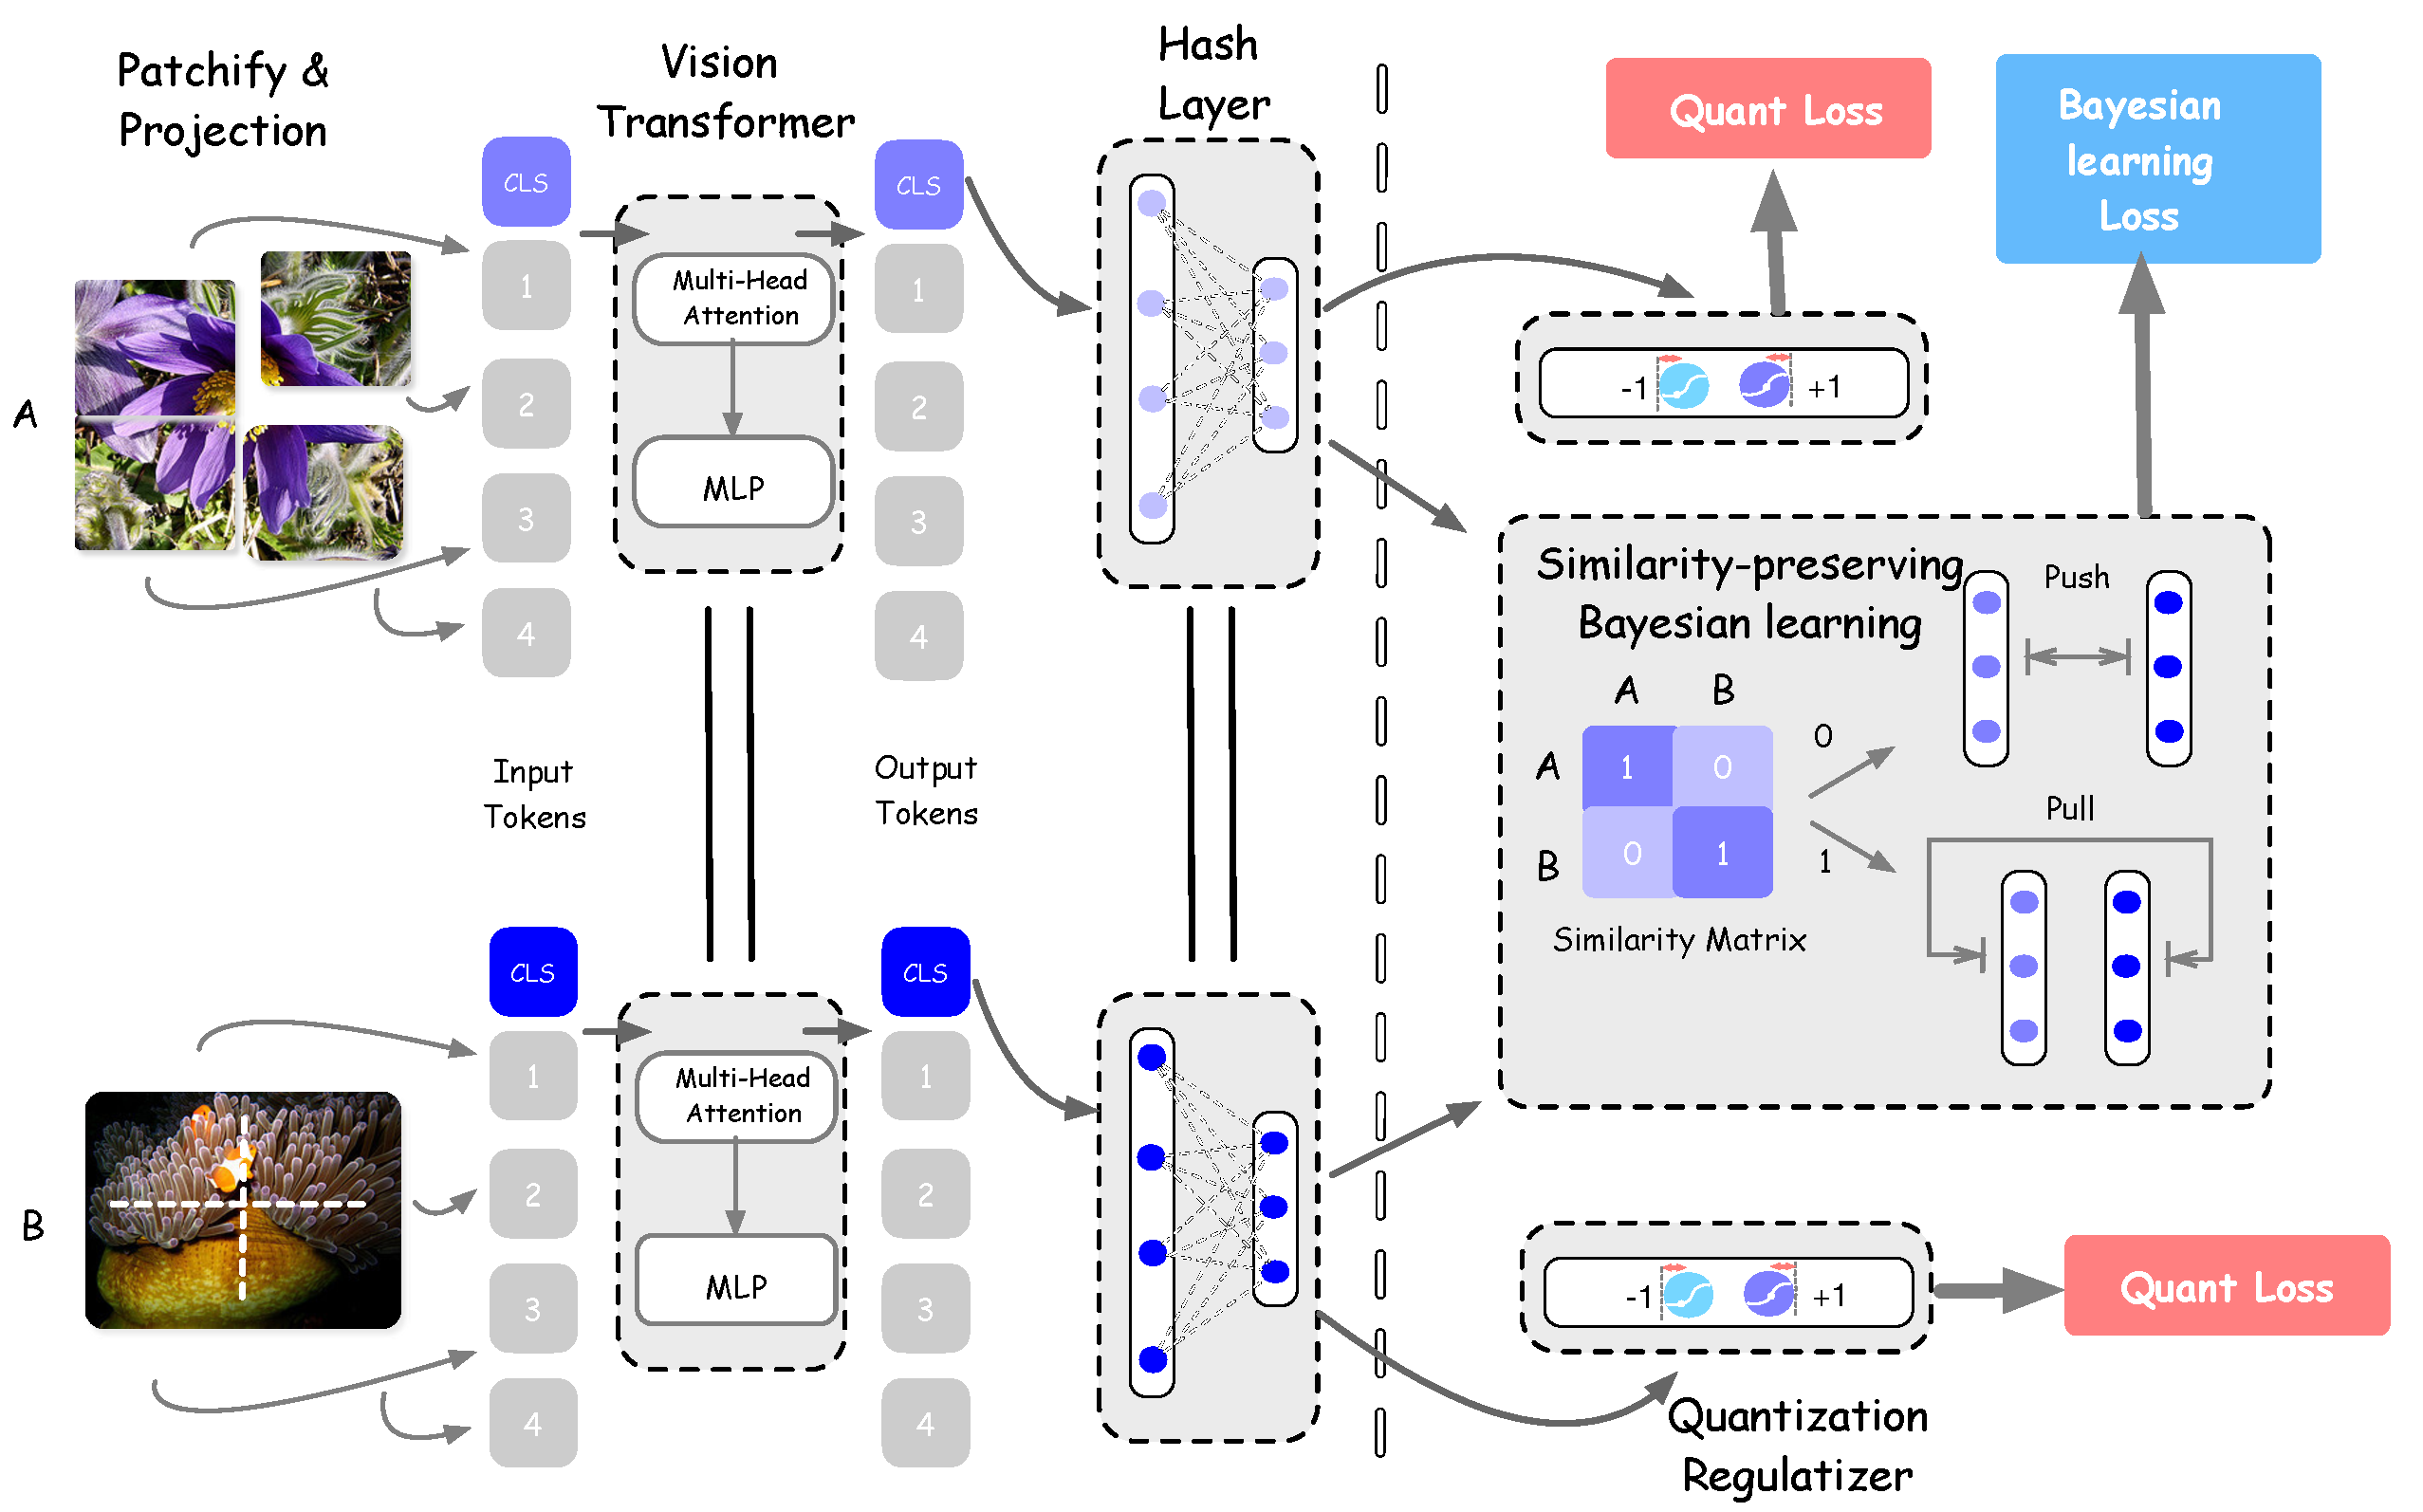
\includegraphics[width=15cm]{04/subfig.pdf} \\
    \bicaption[基于孪生Vision Transformer的图片检索基本框架]
      {对于一个图片对 (A, B), 我们将它们分割成固定大小的多个小图片块。然后将每个小块的像素转变成一个向量并且通过全连接降维成为一系列的嵌入表示。随后, 我们在这一系列的嵌入表征前添加一个随机初始化的向量作为分类嵌入。随后两串表征被输入进孪生Transformer模型并且通过一个哈希层生成$B$为的哈希向量。我们使用基于贝叶斯的学习框架来进行相似度保持学习。}
      {For an image pair (A,B), we cut them into several patches. Then every patch is flattened and projected to a fix-sized embedding with a fully connected layer, resulting in a sequence of embeddings. Subsequently, we add a classification token in the front of each sequence. Then, two sequences are fed into the Siamese transformer architecture. At last, we add a hash layer projecting the feature into B-bit hash vectors. The Bayesian learning module is employed to preserve the similarity in the \textit{Hamming} space for each pair. }
   \label{fig:subfig}
\end{figure} 
基于手工特征的浅层次哈希方法一般是通过基于人工设计的视觉特征描述符来进行哈希函数的学习~\cite{charikar2002similarity, indyk1997locality, weiss2008spectral}, 例如 \textbf{GIST}~\cite{oliva2001modeling}等。经典的浅层次哈希方法有~\textbf{LSH}~\cite{indyk1997locality}, 其主要思想是将相似的高维数据以比较大的概率被映射到相近的哈希编码中。然而由于基于手工提取的特征向量其实并不能准确的刻画保存原图片的有区别性的信息, 这导致了基于手工特征的哈希算法有一道无法逾越的性能鸿沟。为了减轻这个问题的影响, 随着AlexNet~\cite{alexnet}的提出, 基于深度学习的特征提取方法开始成为计算机视觉领域的主流。基于深度学习的模型~\cite{dosovitskiy2020image, russakovsky2015imagenet}相比较基于手工特征的方法通常而言可以获得显著的性能提升。基于深度学习的哈希学习方法一般包含两个阶段。 第一阶段致力于基于深度卷积神经网络, 例如 \textbf{AlexNet}等, 学习有判别性的特征。第二阶段包含设计各种非线性的函数来将连续性的神经网络输出转化成固定的哈希长度的二进制哈希码, 并且通过各种度量学习的损失函数~\cite{cakir2019hashing,cao2018deep,erin2015deep,gong2012iterative, li2015feature}来在汉明空间保存其对应的图片的视觉相似性。 \par
最近, Transformer~\cite{vaswani2017attention}模型展示了其在自然语言领域的卓越性能~\cite{brown2020language, devlin2018bert}。随后, Google设计了 Vision Transformer~\cite{dosovitskiy2020image}, 一种基于 Transformer的变种, 正式将Transformer引入进计算机视觉领域。Vision Transformer 开始在各个计算机视觉任务上超越传统基于卷积神经网络的模型(例如, 图像分类~\cite{dosovitskiy2020image}, 行人重识别~\cite{he2021transreid},等)。如图~\ref{fig:subfig}所示, Vision Transformer 通过首先将输入的图片分割成一系列的2D图片块。 随后, 将图片块转换成向量并且通过可以学习的转换矩阵来将向量降维成低维度的特征表示。 随后, 一系列的输入向量可以被输入进标准的Transformer的编码器架构来学习特征表示。受Vision Transformer的高性能表现的启发, 我们思考完全基于Vision Transformer设计一个深度哈希框架的可行性。\par
在本章中, 我们基于Transformer 设计了一个新型的深度哈希框架-\textbf{TransHash}, 这是有史以来第一个不基于卷积神经网络作为主干网络来进行特征学习的深度哈希架构。具体而言, 为了进行成对的哈希学习, 我们设计了一个孪生多粒度Vision Transformer主干网络 (Multi-Granular Vision Transformer, MGVT)。它包含了两个完全一致的多粒度学习的Transformer网络, 并且这两个网络是完全共享所有参数~\cite{bromley1993signature}。具体而言, 为了进行多粒度的学习, 我们受\textbf{TransReID}~\cite{he2021transreid}所启发, 我们在传统的Vision Transformer的最后一层上设计了一个双流特征学习机制, 将最后一个Transformer块设计成两个并行的分支。对于第一个分支, 它是用来进行全局特征的学习。对于并行的第二个分支, 我们将前一个Transformer块的输出序列进行重新分组成$K$个序列组。这$K$个序列组的序列前都被添加了共享的用于分类的嵌入表征。随后, 将这$K$个序列分别输入进最后一个Transformer层来输出$K$个局部的特征。通过这样的方法, 我们可以通过全局和局部的网络架构设计同时学习到粗粒度的全局特征以及细粒度的局部特征。同时, 我们的模型还可以取得和Lai等人的工作~\cite{lai2015simultaneous}相似的效果。通过将哈希码的表征变成多个分支的哈希码的拼接, 类似于Lai等人提出的 divide-and-encode模块, 可以降低哈希码的冗余性。为了在特征空间保持原来图片的语义相似性, 我们提出采取基于贝叶斯学习的框架来将相似的图片对在特征空间中尽量拉近, 而将不相似的图片在特征空间中尽量拉远。最终, 由于基于卷积神经网络学习到的特征表示是连续的, 我们需要采用\textit{Sign}函数从将连续的表示生成离散的二进制哈希码。但是, 由于离散的哈希码$h$和连续的特征表示$f$之间存在鸿沟, 也就是``量化误差''~\cite{zhu2016deep}的存在, 直接在测试阶段使用\textit{sign}函数只能取得次优的检索性能。为了缩小量化误差, 减轻在测试阶段的性能损失, 我们将相似度保持学习重新规划成一个受限制的优化问题。具体做法是在之前的贝叶斯学习框架后加上一个科西分布量化损失来在训练阶段缩短连续的特征表示和二进制哈希码之间的差距。\par
总结而言, 本章做出了以下的创新与贡献:
\begin{enumerate}
    \item 本章设计了一个基于Vision Transformer的孪生多粒度Vision Transformer主干网络(Multi-Granular Vision Transformer, MGVT)。在传统的Vision Transformer的最后一层, 我们通过将其最后一层设计成一个并行的两个独立的分支, 设计一个新型的双流特征学习框架。 通过这种方法, 我们可以同时学习全局和局部的特征表示。同时, 如前所述, 它也可以进一步提高最后学习到的哈希向量各个位之间的独立性。
    \item 通过采用一个基于贝叶斯的相似度保持的贝叶斯学习模块以及一个量化损失的限制, 我们实现了第一个完全基于Transformer的深度哈希框架-\textbf{TransHash}来进行大规模的图像检索。据我们所知, 这是第一个不基于卷积神经网络的进行大规模图像检索的深度哈希框架。
    \item 我们在三个标准的检索数据集-\textbf{CIFAR-10}, \textbf{NUSWIDE} 和~\textbf{IMAGENET}-设计并且进行了一系列的全面的实验。实验结果表明了本章提出的框架-\textbf{TransHash}-具有优越的性能表现, 相比较当时的深度哈希算法而言可以获得明显的性能提升。
\end{enumerate}

\section{相关工作}
在本小节,~我们介绍与本章工作相关的其他工作。我们将相关的工作分为三个类别: (1) 在计算机视觉领域卷积神经主干网络的发展 (2) 在计算机视觉领域的Transformer的进展 (3)图像检索的深度哈希相关工作。
\subsection{计算机视觉领域的卷积神经网络发展}
卷积神经网络一开始是由LeCun 等人~\cite{cnnoriginal}提出来进行手写数字的自动识别。它提出了卷积核来对图片像素在空间区域的联系进行建模从而提取特征, 并且取得了显著的识别性能。然而直到2012年, \textbf{AlexNet}~\cite{alexnet}的提出, 基于卷积神经网络的方法才开始成为计算机视觉领域绝大部分任务的主要模型, 例如``实例分割''~\cite{he2016deep, ren2017end}, ``图像修复''~\cite{yeh2017semantic,yu2019free}, ``深度哈希''~\cite{cao2018deep, cao2017hashnet}, ``行人重识别''~\cite{chen2020maenet, hermans2017defense, ye2018hierarchical, ye2018visible} 等等。为了提高卷积神经网络的表征能力, 一系列更加深更加有效的卷积神经网络被提出。2014年, Simonyan and Zisserman~\cite{simonyan2014very} 提出了 VGG 网络。 VGG 从网络结构深度的角度来提升CNN的性能。通过使用3*3的小尺寸卷积核作为所有卷积层的标准, VGG 包括了最低11层到最高19层 (VGG-11、 VGG-13、 VGG-16、 VGG-19)等变种, 证明了提高模型的深度可以更好的学习图像中的视觉特征。 随后 GoogLeNet~\cite{szegedy2015going} 提出同时学习多尺度的图像特征。通过使用同时使用不同大小的卷积核(5*5、3*3、1*1)对图像进行卷积操作, 以及在通道维度进行拼接, 可以学习不同粒度的图像特征。在卷积神经网络发展的同时, 研究人员发现一味的增加卷积神经网络的深度在某个时候不能增加模型的性能, 甚至会导致梯度消失或者梯度爆炸等问题, 从而导致模型退化。为了解决这个难题, 2015年, Kaiming~\cite{he2016deep} 提出~\textbf{ResNet}, 通过恒等映射和残差映射来解决梯度消失的问题。从此,~\textbf{ResNet}开始成为计算机视觉领域的一个标准的基础主干神经网络。尽管基于卷积神经网络的模型目前任然在视觉领域占据主要的部分, 最近Vision Transformer的出现开启了采取Transformer的架构来进行一系列的视觉任务的可能性。本章提出的算法在当时是第一批利用Transformer来解决经典计算机视觉领域任务的工作。\par
\subsection{计算机视觉领域的Transformer发展}
Transformer最初是有2017年Google提出~\cite{vaswani2017attention}, 在自然语言处理领域进行序列数据的处理。从那时开始, 许多科研人员就开始在研究Transformer架构在计算机视觉领域的效果。最初的做法是利用Transformer处理由卷积神经网络提取的序列化的特征图~\cite{carion2020end, girdhar2019video, xie2021segmenting}。在2020年, Google提出了\textbf{Vision Transformer} (ViT) 通过将图片数据分块然后通过线性映射转换成一个序列的向量然后直接输入进传统的Transformer里通过在大型数据集上预训练后,就可以在多个任务如图像分类等领域取得了接近\textbf{ResNet}的性能。随后不同的ViT的变种开始在计算机视觉多个任务取得超越\textbf{ResNet}的性能效果。DeiT~\cite{touvron2021training}~是一个证实Transformer可以在中等大小的数据集上进行预训练并且取得较有的性能。DeiT通过使用CNN的输出当做一个教师模型, 通过蒸馏学习(Distillation Learning)来帮助训练自身的Transformer架构。在输入的嵌入表征前, 它们添加了一个蒸馏表征, 然后通过交叉熵损失和蒸馏损失进行训练。随后 Token-to-Token (T2T) Vision Transformer~\cite{yuan2021tokens}递归的将临近的token融合成一个token来降低序列的长度并且对于空间中的较远的联系进行建模。 Transformer in Transformer~\cite{han2021transformer}提出在两种层面上进行其中关键的注意力操作: (1) patch 层面, 与传统的ViT类似。 (2) 局部子patch层面, 通过将多个patch组合成一个大的子patch进行自注意力机制计算。通过这样的机制, 模型可以学习到更加细粒度的特征,~取得了更加优异的性能。由于ViT中的自注意力机制的计算复杂度对于输入的序列长度而言是 $O(n^2)$, 这极大的限制了模型的可应用性。Pyramid ViT (PVT)~\cite{wang2021pyramid} 提出一个分层次的ViT设计, 通过逐步将整合临近的token缩小自注意力机制计算的序列长度。随后2021年的ICCV最佳论文~Swin Transformer~\cite{liu2021swin}通过将输入的图片块分成一个个限定大小窗口, 并且只在窗口内进行自注意力的计算。为了建立不同窗口内的patch之间的联系, 作者提出了一个Shifted Window分割机制, 在连续的两个Transformer层之间进行基于window的自注意力计算和shifted window的自注意力计算。Swin Transformer 在多个计算机视觉领域取得超越传统基于\textbf{ResNet-50}的模型, 开始成为取代卷积神经网络的计算机视觉主干深度神经网络。随后, CrossFormer
也基于一个分层次的Pyramid架构提出short-distance 注意力和long-distance 注意力, 在降低计算复杂度的同时可以同时捕捉局部和全局的特征信息。RegionVit~\cite{chen2021regionvit} 提出一个regional-to-local的注意力机制来对层次性特征进行编码。\par
除了上述基于ViT的基础主干网络的发展, 基于ViT的计算机视觉任务的应用也以惊人的速度增长。例如在``目标检测''任务中, Fang 等人提出~\cite{fang2021you}一个完全基于Transformer的目标检测框架。它将ViT中的用于分类的token替换成了多个可以学习的目标查询的token。在``图像分割''领域, Segmentation Transformer (SETR)~\cite{zheng2021rethinking} 使用ViT作为编码器, 使用两个解码器进行逐步的上采样。随后 SegFormer~\cite{strudel2021segmenter}~使用一个基于Pyramid ViT的编码器和一个简单的基于MLP的解码器来得到分割的掩膜。同样, Transformer在低层次视觉任务方面也取得了卓越的表现。在``图像处理''方面, chen 等人提出了一个基于预训练的Transformer模型。它可以进行多种图像修复的工作, 例如图像超分, 图像去噪, 等。除了在传统2D视觉领域, Transformer在3D计算机视觉方向也取得了令人瞩目的效果。3D点云的排序不变的特征天然适合Transformer的计算特性。2021年, Zhao 等人提出了 Point Transformer~\cite{zhao2021point} 提出了一个新型的点云Transformer层来对3D点的局部邻接信息进行自注意力计算。这个Transformer层基于向量自注意力机制, 其中的注意力权重是通过向量来表示。
Guo等人~\cite{guo2021pct}提出Pct来显式的对局部的3D结构进行编码, 并且在3D形状分类, 分割等领域取得了较好的性能表现。Lin等人提出一个Mesh Transformer~\cite{lin2021end}通过2D的图片重建3D得行人姿态以及进行网格重建, 这是第一个基于Transformer的3D行人重建的工作, 并且也取得了较好的结果。\par
Vision Transformer在此时仍然处于研究的初期, 并且由于其优越的性能得到了各个研究机构以及工业界的持续性上涨的关注。越来越多的研究人员在讲Vision Transformer引入进自己的研究方向来解决实际的问题。

\begin{figure}[!htp]
    \centering
    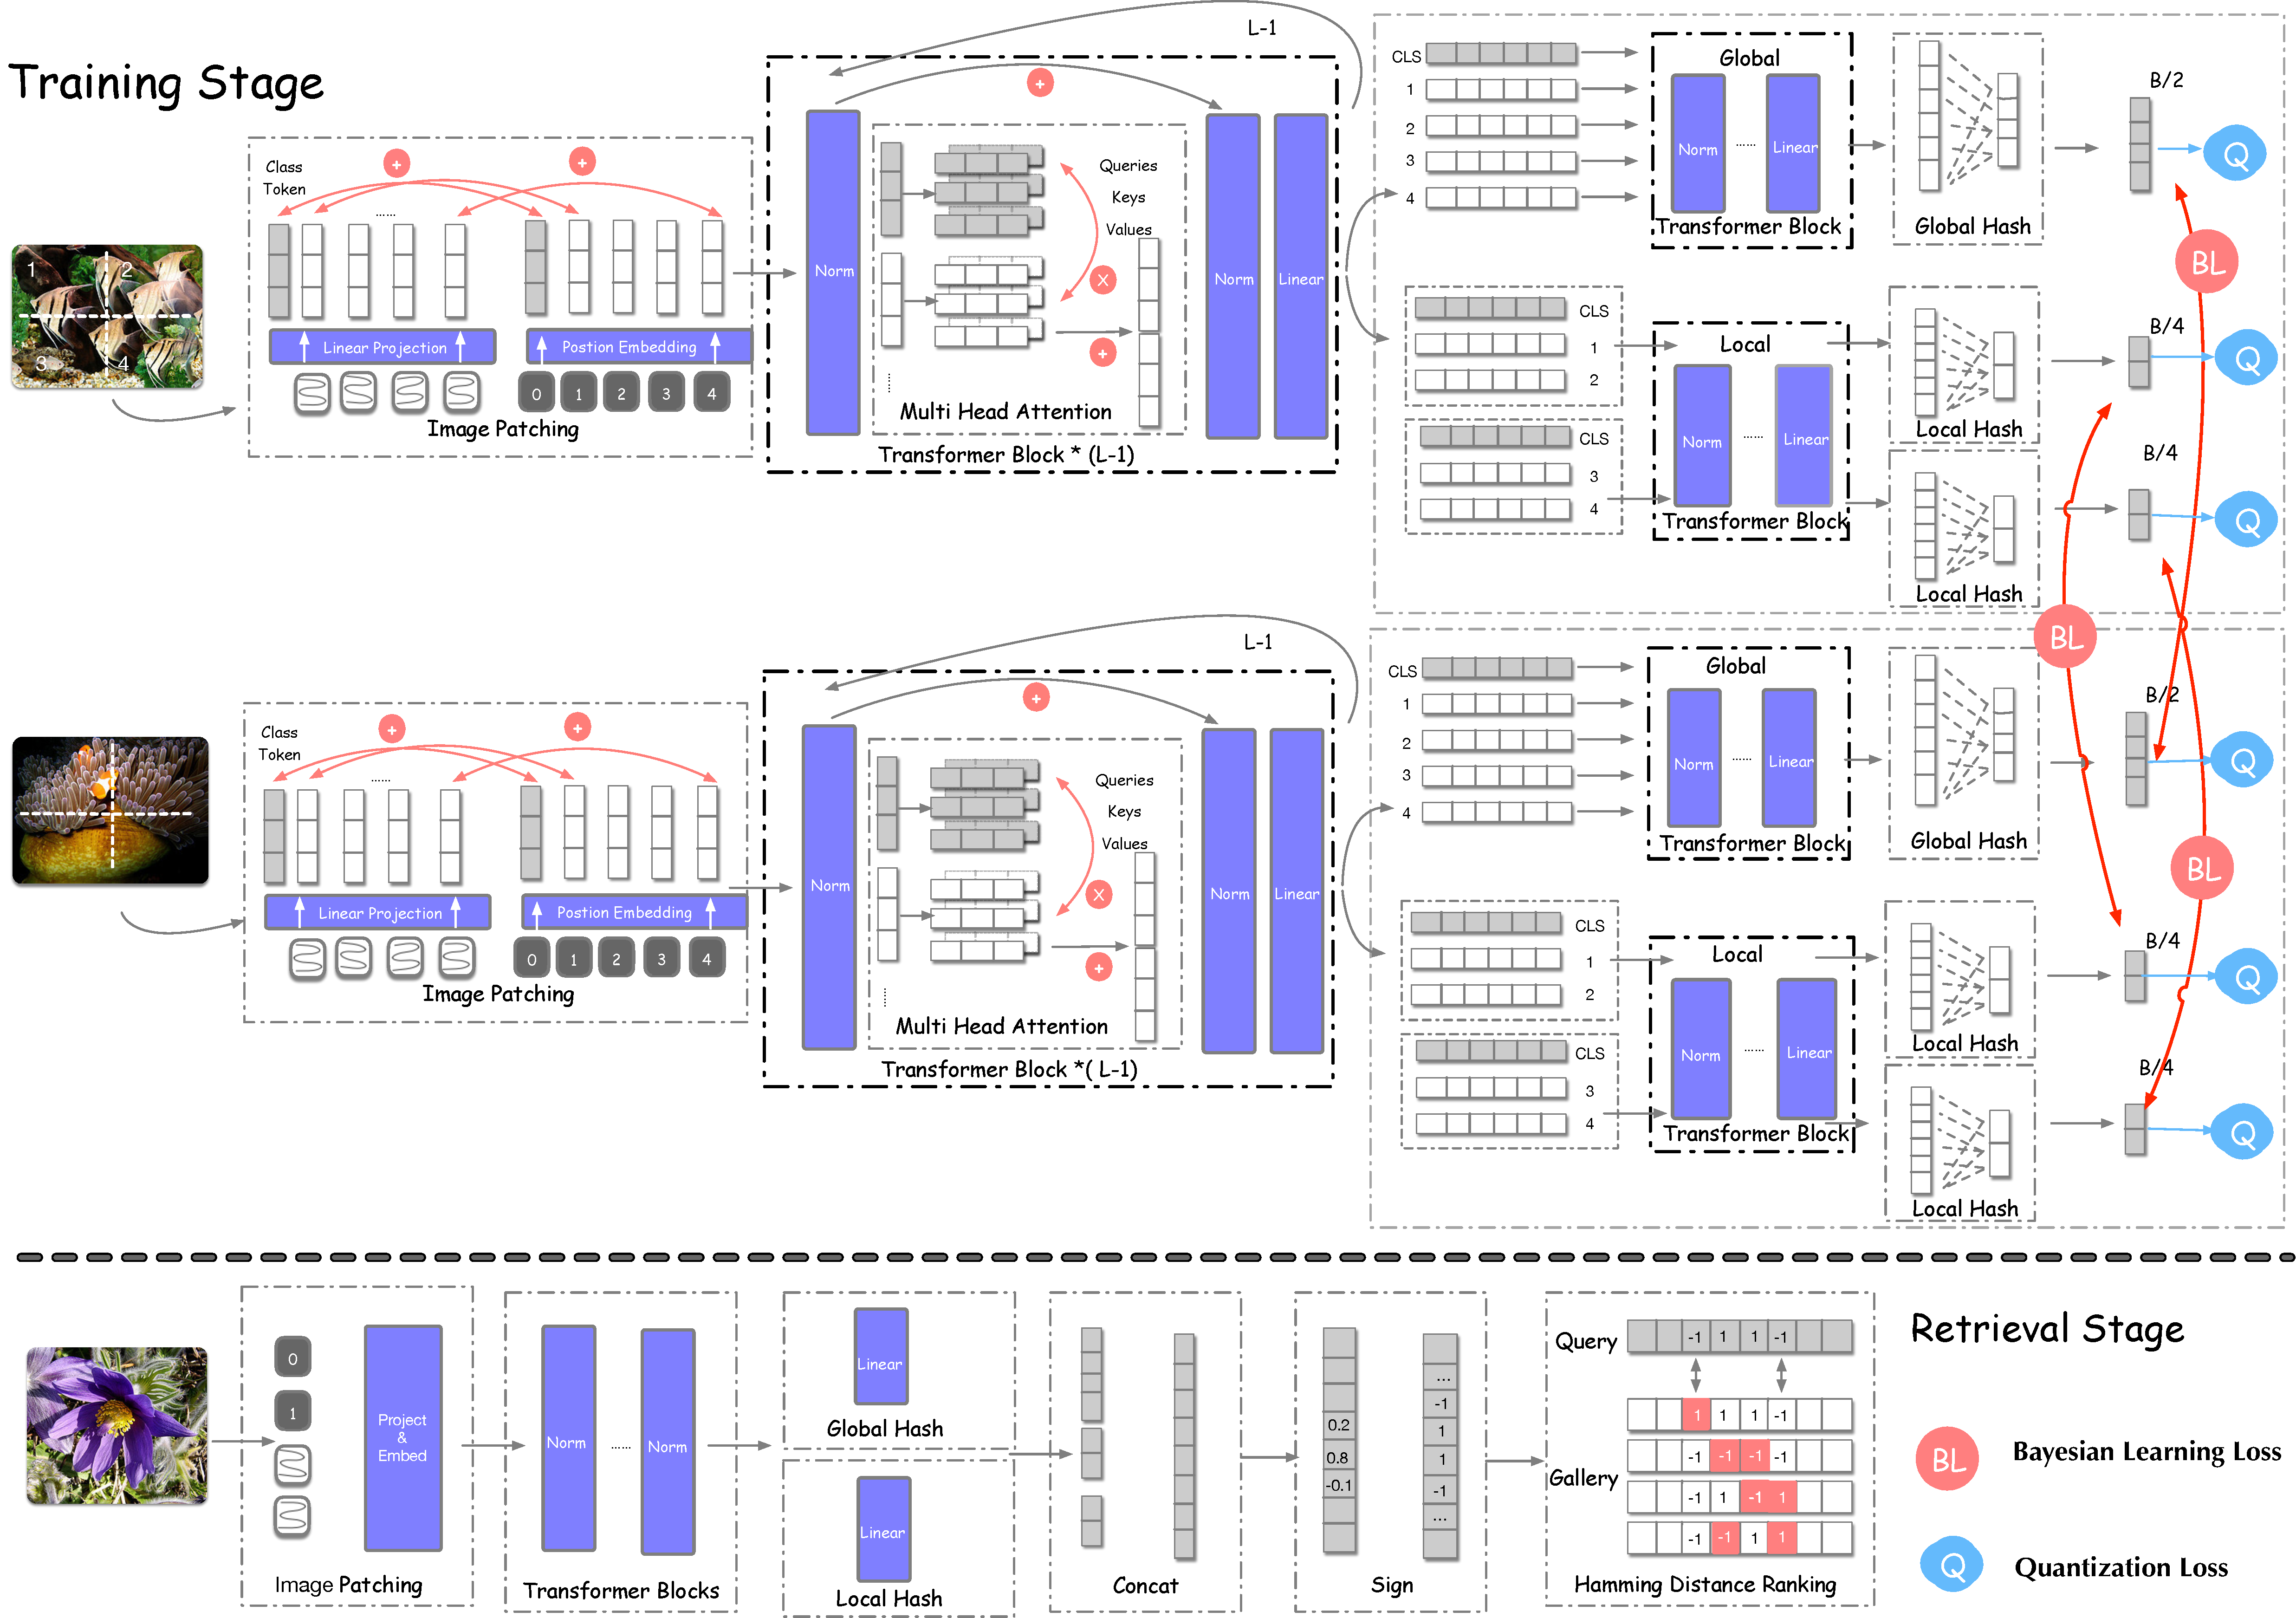
\includegraphics[width=15cm]{04/architecture.pdf} \\
    \bicaption[基于Vision Transformer的深度哈希框架]
      {TransHash的细节框架。图上部分表示了框架进行训练的阶段。我们采用一个孪生的架构。如传统的ViT, 输入图片将被切割成多个小块并且降维成一个序列的嵌入表征。在Transformer的最后一层, 我们设计了两个并行的Transformer 层来学习全局和局部的信息。同时, 对于全局和局部的特征, 我们均设计了对应的哈希层来进行哈希码的学习。 图的下部分表示测试阶段, 其中全局和局部的哈希码被连接成一个哈希码进行检索。}
      {The detailed architecture of the proposed \textbf{TransHash}. The upper part denotes the training stage. Specifically, we follow the same protocols as ViT by feeding the patch embedding together with the position embedding into the transformer encoder. At the last layer of the transformer, we design two parallel transformer blocks: global and local transformer blocks.  For the global feature and each local feature, we design a corresponding hashing layer. In the testing stage, the global and all the local hash vectors are concatenated and quantized into one hash code.}
   \label{fig:mainarch}
\end{figure} 

\subsection{基于哈希的图像检索}
深度哈希在大规模高效图像检索领域~\cite{chen2021dvhn, ge2013optimized, gong2012iterative, heo2012spherical} \cite{indyk1997locality, yu2018product, weiss2008spectral}近年来获得了越来越多的关注。根据它们提取特征的方法, 我们可以将它们分成两个类别: ``浅哈希方法''和``基于深度学习的哈希方法''。 \par
传统的浅哈希方法一般基于手工设计的特征来学习一个哈希函数将图片映射到二进制哈希码。一个典型的例子是~ Locality Sensitive Hash (LSH)~\cite{indyk1997locality}。LSH 致力于寻找一个哈希族使得相似的对象经过哈希函数产生的哈希碰撞要比不相似的概率要高。随后, Charikar等人~\cite{charikar2002similarity}提出另一个基于LSH的变种, SIMHASH, 其针对在欧式空间中的余弦相似性。 尽管这些基于手工特征的方法取得了一定程度的成功。 但是当应用到现实的数据时, 由于图片具有较多外观变化, 基于手工设计的特征并不能提取到有判别性的信息, 从而导致了哈希精度的不足。\par
基于这一点, 基于深度卷积神经网络提取特征进行哈希学习的方法研究取得了极大的进展~\cite{cao2017hashnet, fan20deep, li2015feature, liu2016deep, zhu2016deep}。2014年, Xia~\cite{xia2014supervised} 提出第一个基于深度学习的监督哈希框架。它提出一种两阶段哈希的方法先将相似度矩阵$S$ 分解成汉明矩阵$H$ 和 $H^T$的乘积, 其中 $H$的每一行代表一个训练图片数据的哈希编码。接着, 卷积神经网络通过第一阶段学习到的哈希码作为监督信号来进行监督训练。Lai等人提出了第一个端到端的深度哈希框架通过三元损失函数以及一个降低哈希码的荣誉性的模块来同时进行特征学习以及二进制哈希码的生成。随后, Zhu~\cite{liu2016deep}提出一个基于贝叶斯学习的框架通过成对的图片数据进行相似度保留学习。HashNet~\cite{cao2017hashnet} 提出使用$tanh(\beta z)$函数, 通过逐步的增大参数$\beta$, 使得神经网络的输出接近二值化, 从而减少测试阶段和训练阶段的量化误差。2018年, Cao等人提出 DCH~\cite{cao2018deep} 使用一个Cauchy分布来替代DHN框架中的sigmoid函数来生成两个图片对的相似度评分。Fan 随后提出 DPN~\cite{fan2020deep} 通过一个深度极化损失(Polarized Loss)来监督模型进行二进制哈希码的生成, 使得不再需要加入常用的量化损失函数来控制模型的输出和量化后的二进制码的误差。传统的深度哈希算法均是基于卷积神经网络而构造。卷积神经网络由于加入了较多对于图片模块的先验信息, 例如图片空间区域接近的地方信息类似, 即具有空间局部性, 导致有较高的归纳偏置~(Inductive Bias)。而Transformer则归纳偏置则较小, 在大量数据进行训练的条件下可以取得优异的性能表现。本章作为第一个探究完全基于Transformer的深度哈希方法, 取得了相比较卷积神经网络更加令人瞩目的性能。

\section{基于Vision Transformer的深度哈希算法}
\subsection{本章主要符号定义以及问题定义}
在本章中, 我们使用书法大写字母 (Calligraphic Uppercase), 例如 $\mathcal{H}$ 来表示映射函数。我们使用粗体大写字母 (Bold-face Uppercase) 如 $\mathbf{T}$ 来代表集合. 粗体小写字母如 $\mathbf{b}$在全章中代表向量。我们使用斜大写字母 (Italic Uppercase)来代表图片, 如 $\textit{I}$。 同时, 在全章中, sign激活函数直接由 $\textit{sign}$ 来表示。\par
\textbf{问题定义:} 假设我们有一个训练数据集$T = \{I_i\}_{i=1}^{NT}$, 包含$NT$张训练数据图片, 以及其对应的监督标签集合 $Y = \{y_i\}_{i=1}^{NT}$。对于在所有的训练数据中的图片对, 我们可以创建一个相似度矩阵$\mathbf{S}$, 其中$s_{ij} = 1$ 如果图片$\it{I}_i$和图片$\it{I}_{ij}$是来自一个类别, 否则的话$s_{ij} = 0$。进行图片检索的深度哈希的目标是学习到一个非线性的哈希函数$\mathcal{H}: \mathbf{I} \mapsto \{0,1\}^B $, 将输入的图片$\it{I}_i$映射到一个二进制的$B$位的哈希向量$\mathbf{h}_i$。其中$\mathbf{h}_i$需要保存在$\mathbf{S}$中的图片之间的相似度信息。也就是说, 如果$s_{ij} = 1$时, $\mathbf{h}_i$和$\mathbf{h}_j$之间的汉明距离应该尽量小。而, $s_{ij} = 0$时, $\mathbf{h}_i$和$\mathbf{h}_j$之间的汉明距离则应该尽量大。

\subsection{孪生Vision Transformer架构}
本章提出的架构如图~\ref{fig:mainarch}所示。对于一个图片对$(\it{I}_i, \it{I}_j)$, 其中每张图片的大小为$H \times W \times 3$, 我们将其切割成多个相同大小的小patch, 其中每个patch的大小为$P \times P \times 3$。通过这样的方法, 我们一共可以得到$N$个patch, 其中  $N = H \times W / P^2$。值得注意的是$N+1$则是输入进Transformer的有效的输入序列长度。 \par
\textbf{Patch 编码} \quad 对于每一个大小为$P \times P \times 3$的图片patch, 我们将其拉平成一个大小为$P^2 \times 3$的向量。随后, 类似于传统的ViT, 我们通过一个全连接神经网络将每一个向量映射到一个$D$维的向量。这样生成了一个序列$\{x_p^k\} \in \mathbb{R}^{D}, k \in [1, N]$。 随后, 我们在序列的前面添加一个可以训练的嵌入向量$x_{class}$。 其对应的状态在Transformer的最后一层的输入是充当用于分类的图片的全局表征。 通过这种方法, 我们得到了最终的输入表征$X_p \in \mathbb{R}^{(N+1) \times D}$。\par
\textbf{位置编码} \quad 位置编码 (positional embedding) 是用来对patch编码增加其对应在2D图片中的位置信息。通过这样的方式, Transformer可以学习到图片块在原图中的空间位置信息。 我们采取ViT的方法, 在序列中的每一个嵌入向量上叠加一个可以训练的位置向量。因此, Transformer第一层的输入$z_o $可以被正式描述为:
\begin{equation}
    z_0 = X_p + E_{pos} = [x_{class}; x_p^1 , ... , x_p^N ] + E_{pos}.
\end{equation} \par
\textbf{基于自注意力的编码器} \quad
Transformer编码器包含$L-1$层, 每一层包含了一个多头的自注意力模块(Multi-headed Self-attention, MHA)和一个多层感知器(Multi-layer Perceptron, MLP)。在每一层前加入一个层次标准化。同时采取残差连接进行每一层的相连, 如图~\ref{fig:mainarch}所示。Transformer的每一层计算如下述公式所示:
\begin{equation}
    \begin{split}
        z_{l} &= \mathcal{F}_{msa}(\mathcal{F}_{ln}(z_{l-1})) + z_{l-1}   \\
      z_{l} &= \mathcal{F}_{mlp}(\mathcal{F}_{ln}(z_{l} )) + z_{l} \\
      \text{where} \\ l & = 1 ... (L-1)
    \end{split}
  \end{equation} \par
\textbf{双流特征学习}\quad 类似于TransReID~\cite{he2021transreid}, 在上述的编码器后, 我们可以得到$Z_{L-1} = [z_{L-1}^0;z_{L-1}^1,z_{L-1}^2, ... ,z_{L-1}^N]$。值得注意的是, $z_{L-1}^0$是对于添加的用于分类的可学习的嵌入表征$x_{class}$的隐向量。受TransReID~\cite{he2021transreid}所启发, 我们设计了两个并行的分支, 用于学习全局特征信息的分支$\mathcal{F}^g_{block}$和用于学习局部特征信息的分支 $\mathcal{F}^l_{block}$。对于全局信息的分支, 它和传统的Transformer层类似,将 $Z_{L-1}$编码成$Z_{L} = [\mathbf{f}_g;z_L^1,z_L^2, ... ,z_L^  N]$, 其中$\mathbf{f}_g$被视作全局特征的代表向量。对于学习局部特征信息的分支, 我们将 $Z_{L-1}$ 分成$K$个组, 并且将一个共享的token $z_{L-1}^0$ 添加在每个组的前部。 通过这样的方法, 我们得到了$K$个输入序列, 如$ \{[z_{L-1}^0;z_{L-1}^1,...,z_{L-1}^{N/K}],$ $ [z_{L-1}^0;z_{L-1}^{N/K+1},...,z_{L-1}^{2\times N/K}], [z_{L-1}^0;z_{L-1}^{N-N/K+1}$ $,...,z_{L-1}^N]\}$所示。随后, 我们将$K$个特征组输入到 $\mathcal{F}^l_{block}$ 来学习$K$个局部的特征向量$\{\mathbf{f}_l^1,\mathbf{f}_l^2,...,\mathbf{f}_l^K\}$。\par
\textbf{哈希神经网络层}
为了学习到紧凑的哈希编码, 我们额外设计了几个哈希层来将特征向量映射成不同长度的哈希向量。具体来说, 假设在检索阶段每一张图片的哈希码长度为$B$, 则对于长度为$M$的全局特征向量, 我们经过映射后得到一个长度为$B/2$的全局哈希向量, 具体的计算如下所示:
\begin{equation}
    h_g = \mathcal{F}_h^g(f_g) = \mathbf{f}_g W^T + b.
\end{equation}
其中$W$是一个大小为$(B/2,M)$的权重矩阵, 而 $b$则是一个偏差权重向量, 其大小为$(B/2,)$。通过同样的方法, 对于每一个局部特征向量 $\mathbf{f}_l \in \{\mathbf{f}_l^1,...,\mathbf{f}_l^K\}$, 我们都设计一个对应的基于全连接的哈希网络层, 其输出维度为 $B/(2*K)$。这样我们可以获得$K$个局部的哈希向量$\{h_l^1,...,h_l^K\}$。 \par
通过这样的方法, 对于每一个图片对$\it{I}_i, \it{I}_j$, 本章的孪生的深度哈希模型输出两个哈希向量集合:  $\{\{h_g\}^i,\{h_l^1\}^i,...,\{h_l^K\}^i\}$ 和 $\{\{h_g\}^j,\{h_l^1\}^j,$ $..., \{h_l^K\}^j\}$。
\subsection{基于贝叶斯的相似度保留学习}
在本章中, 我们提出基于一个贝叶斯学习的框架进行相似度保留的深度哈希训练。给定一对训练数据图片对$(\it{I}_i,\it{I}_j,s_{ij}): s_{ij} \in \textbf{S}$, 其中 $s_{ij} =1 $ 如果 $\it{I}_i$和 $\it{I}_j$是来自于同一个类别。相反, 则 $s_{ij} =1 $。我们可以用公式描述基于哈希码的$\boldsymbol{H} = \{ \mathbf{h}_1, \mathbf{h}_2,...,\mathbf{h}_P\}$的最大先验估计为:
\begin{equation}
    \begin{aligned}
    \log P(\boldsymbol{H} \mid \mathbf{S}) & \propto \log P(\mathbf{S} \mid \boldsymbol{H}) P(\boldsymbol{H}) \\
    &=\sum_{s_{i j} \in \mathbf{S}} w_{i j} \log P\left(s_{i j} \mid \boldsymbol{h}_{i}, \boldsymbol{h}_{j}\right)+\sum_{i=1}^{NT} \log P\left(\boldsymbol{h}_{i}\right).
    \end{aligned}
    \label{eq:map}
\end{equation}
其中 $P(\mathbf{S} \mid \boldsymbol{H})$是一个带权的似然函数, $w_{ij}$则是对于每一个图片对 $(I_i,I_i)$的对应的权重。相似性矩阵$\mathbf{S}$在现实的检索场景中非常的稀疏~\cite{cao2017hashnet}, 这通常会导致数据不平衡的问题, 从而导致检索性能的下降。 我们采用带权重的似然函数对每一个图片对分配一个对应的权重来解决这个问题, 如下所示:
\begin{equation}
    w_{i j}=\left\{\begin{array}{ll}
|\mathbf{S}| /\left|\mathbf{S}_{1}\right|, & s_{i j}=1 \\
|\mathbf{S}| /\left|\mathbf{S}_{0}\right|, & s_{i j}=0
\end{array}\right.
\end{equation}
其中$\mathbf{S}_{1}=\left\{s_{i j} \in \mathbf{S}: s_{i j}=1\right\}$ 是属于同一个类别的图片对的集合。而$\mathbf{S}_{0}=\left\{s_{i j} \in \mathbf{S}: s_{i j}=0\right\}$ 则是不属于同一个类别的图片对的集合。对于每一对哈希向量对 $(\mathbf{h}_i,\mathbf{h}_j)$, $P\left(s_{i j} \mid \boldsymbol{h}_{i}, \boldsymbol{h}_{j}\right)$ 则是一个给定一对哈希码$\mathbf{h}_i$和$\mathbf{h}_j$后对于$s_{ij}$的条件概率。因为$s_{ij}$的取值为二值, $0$和$1$, 我们自然可以将$P\left(s_{i j} \mid \boldsymbol{h}_{i}, \boldsymbol{h}_{j}\right)$定义为一个伯努利分布(Benoulli Distribution):
\begin{equation}
    \begin{aligned}
P\left(s_{i j} \mid \boldsymbol{h}_{i}, \boldsymbol{h}_{j}\right) &=\left\{\begin{array}{ll}
\sigma\left(\mathcal{D}_H\left(\boldsymbol{h}_{i}, \boldsymbol{h}_{j}\right)\right), & s_{i j}=1 \\
1-\sigma\left(\mathcal{D}_H\left(\boldsymbol{h}_{i}, \boldsymbol{h}_{j}\right)\right), & s_{i j}=0
\end{array}\right.\\
&=\sigma\left(\mathcal{D}_H\left(\boldsymbol{h}_{i}, \boldsymbol{h}_{j}\right)\right)^{s_{i j}}\left(1-\sigma\left(\mathcal{D}_H\left(\boldsymbol{h}_{i}, \boldsymbol{h}_{j}\right)\right)\right)^{1-s_{i j}}.
\end{aligned}
\label{eq:beyesian}
\end{equation}
其中$\mathcal{D}_H(.)$是一个汉明距离函数, $\sigma$是一个概率函数, 其通过输入一对哈希码的汉明距离然后输出一个他们来自于同一个类别的概率。 由于直接优化离散的哈希码是一个极其有挑战的问题, 我们在训练阶段对二进制的哈希码$\mathbf{h}_i \in \{-1,1\}^B$使用持续性放松, 类似于之前的工作~\cite{cao2017hashnet,cao2018deep,zhu2016deep}。因此, 在连续的空间, 我们可以采用一个对于$\mathcal{D}_H(.)$的替代 $\mathcal{D}_S$来进行距离的计算, 如下所示:
\begin{equation}
    \begin{aligned}
    \mathcal{D}_S\left(\boldsymbol{h}_{i}, \boldsymbol{h}_{j}\right) &=\frac{K}{4}\left\|\frac{\boldsymbol{h}_{i}}{\left\|\boldsymbol{h}_{i}\right\|}-\frac{\boldsymbol{h}_{j}}{\left\|\boldsymbol{h}_{j}\right\|}\right\|_{2}^{2} \\
    &=\frac{K}{2}\left(1-\cos \left(\boldsymbol{h}_{i}, \boldsymbol{h}_{j}\right)\right)
    \end{aligned}    
    \label{eq:prob}
\end{equation}
对于概率函数$\sigma(.)$, 最常使用的函数是$sigmoid(.)$函数。然而, 如Cao等人之处~\cite{cao2018deep}指出, 其输出的概率在输入的汉明距离远大于$2$是一个较稳定的高值。只有当输入的汉明距离接近$b/2$时候, 概率才开始下降。这个特性使得基于$sigmoid(.)$的深度哈希方法很难将相似对的距离降低到一个较低的程度。考虑到这一点, 我们提出基于一个柯西分布的概率函数, 如下所示:
\begin{equation}
    \sigma\left(\mathcal{D}_S\left(\boldsymbol{h}_{i}, \boldsymbol{h}_{j}\right)\right)=\frac{\gamma}{\gamma+\mathcal{D}_S\left(\boldsymbol{h}_{i}, \boldsymbol{h}_{j}\right)}
\label{eq:cauchy}
\end{equation}
其中 $\gamma$是一个代表了柯西分布的等级的超参数。柯西分布有一个较好的特性, 其概率输出在汉明距离较低的情况下依然可以下降陡峭, 这使得其可以将相似图片对的汉明码距离拉近到一个较小的半径中。通过将公式~\ref{eq:cauchy},~公式~\ref{eq:prob}以及公式~\ref{eq:beyesian}输入进最大先验估计(\textbf{MAP})的模型中, 我们可以得到如下的优化目标:
\begin{equation}
    \begin{aligned}
         L_{s} &= \sum_{s_{i j} \in \mathbb{S}} L_{ce}(\boldsymbol{h}_i,\boldsymbol{h}_j) \\
         &=\sum_{s_{i j} \in \mathbf{S}} w_{i j}\left(s_{i j} \log \frac{\mathcal{D}_s\left(\boldsymbol{h}_{i}, \boldsymbol{h}_{j}\right)}{\gamma}+\log \left(1+\frac{\gamma}{\mathcal{D}_S\left(\boldsymbol{h}_{i}, \boldsymbol{h}_{j}\right)}\right)\right)
    \end{aligned}
    \label{eq:final}
\end{equation}
从公式~\ref{eq:beyesian}和公式~\ref{eq:final}, 我们可以发现 $L_{s}$具有一个类似于逻辑回归的形式。通过优化$L_{s}$,  对于一对来自于同一个类别的图片对$(I_i,I_j)$, 我们会增大$P(1|\textbf{h}_i,\textbf{h}_j)$。由于$\sigma(.)$是一个单调递减的柯西函数, 这会导致这对图片对应的哈希向量的汉明距离$\mathcal{D}_S(\mathbf{h}_i, \mathbf{h}_j)$的增大。\par
为了缩小在训练阶段的连续性的哈希向量和其对应的二值化的二进制哈希码之间的差距, 我们可以从提出的先验分布中推导出我们的量化损失函数。
\begin{equation}
    P\left(\boldsymbol{h}_{i}\right)=\frac{\gamma}{\gamma+\mathcal{D}_S\left(\left|\boldsymbol{h}_{i}\right|, \mathbf{1}\right)}.
\end{equation}
其中$\mathbf{1}$是一个所有维度都是1的向量, 而$\gamma$则是和公式~\ref{eq:cauchy}一致的超参数。因为在 公式~\ref{eq:map}中我们实际上需要最大化$P(H)$, 相对应则可以得到量化损失函数为: 
\begin{equation}
    L_Q =  \sum_{i=1}^{NT} Q(\boldsymbol{h}_i)=\sum_{i=1}^{NT} \log \left(1+\frac{\mathcal{D}_S\left(\left|\boldsymbol{h}_{i}\right|, \mathbf{1}\right)}{\gamma}\right).
\label{eq:quant}
  \end{equation}
通过最小化$L_Q$, 哈希向量$\mathbf{h}$的每一个维度都被驱使接近$1$或者$-1$, 从而获得接近二值化的哈希码。
\subsection{端到端的训练}
在这一小节中, 我们接受本章提出的\textbf{TransHash}的优化目标函数。 给定成对的训练图片数据集
$(I_i,I_j)$, 我们可以通过将图片对输入进孪生Vision Transformer得到一对连续的哈希向量集合$\{\{h_g\}^i,\{h_l^1\}^i,...,\{h_l^K\}^i\}$ 和 $\{\{h_g\}^j,\{h_l^1\}^j$ $,...,\{h_l^K\}^j\}$。随后, 对于局部的特征, 我们可以得到相似度保持的贝叶斯损失和量化损失如下所示:
\begin{equation}
    \begin{aligned}
        L_{B}^{local} = \sum_{s_{i j} \in \mathbf{S} } \sum_{k}^K L_{ce}(\{\textbf{h}_l^k \}^i,\{\textbf{h}_l^k \}^j) \\
        L_{Q}^{local} = \sum_i^{NT} \sum_j^K Q(\{h_l^j\}^i)
    \end{aligned}
    \end{equation}
其中$N$是训练数据集中图片的总数, $\mathbf{S}$代表相似度矩阵, $K$是代表每一张图片的局部特征的数量。 用相同的方法我们可以得到全局的损失函数为:
\begin{equation}
    \begin{aligned}
        L_{B}^{global} = \sum_{s_{i j} \in \mathbf{S} }  L_{ce}(\{\textbf{h}_l^k \}^i,\{\textbf{h}_l^k \}^j) \\
        L_{Q}^{global} = \sum_i^{NT} Q(\{h_l^j\}^i)
    \end{aligned}
    \end{equation}
总共的训练目标函数如下式所示:
\begin{equation}
    \min_{\theta} L_B^{global} + L_B^{local} + \lambda (L_Q^{global} + L_Q^{local})
\end{equation}
其中$\theta$表示框架中可以学习的参数, 而 $\lambda$代表控制柯西量化损失函数的重要性的超参数。
\subsection{大规模的检索阶段}
在这小节, 我们阐述如何利用训练好的\textbf{TransHash} 进行高效的大规模图像检索。通常我们给定一个查询的数据集$\mathbf{Q}$和一个数据库数据集$\mathbf{G}$。 对于每一张查询图片 $\it{I}^q_{k}$, 我们可以得到对应的二进制哈希向量如下:
\begin{equation}
    \mathbf{b}^q_k = \textit{sign}([\{h_g\}^i,\{h_l^1\}^i,...,\{h_l^K\}^i])
\end{equation}
随后通过这种方式, 对于在$\mathbf{G} = \{\it{I}^g_k\}_{k=1}^{N_g} $,  我们可以获得二进制一个哈希码集合:$\mathbf{H^g} = \{\mathbf{b}_k^g\}_{k=1}^{N_g}$。随后通过使用查询图片的哈希码$\mathbf{b}^q_k$和$\mathbf{H^g} $每个哈希码进行汉明距离的计算, 可以根据数据库中图片于查询的图片的哈希码的汉明距离进行由小到大排序来进行检索。

\section{实验结果与分析}
在这个章节, 我们仔细的评估测试了\textbf{TransHash}在标准的大规模图像检索数据集上的性能, 并且与先进的其他算法进行了细致的对比。我们首先给出简要的介绍和我们模型的实现细节,数据集的具体信息以及评估指标。随后, 我们展示了详细的实验结果分析以及对比。
\begin{table}[!htpb]
    %% \centering % not needed
    \bicaption{各个先进深度哈希算法在\textbf{CIFAR-10}上的测试结果}{Results of state-of-the-art deep hashing methods on \textbf{CIFAR-10}}
    \centering
    \begin{tabular}{cccccc}
       \\ \hline
    \multicolumn{2}{l|}{Methods} & 16-bit & 32-bit & 48-bit & 64-bit   \\\hline
    \multicolumn{2}{l|}{SH~\cite{weiss2008spectral} (NeurIPS)} & - & - & - & -  \\  
    \multicolumn{2}{l|}{ITQ~\cite{gong2012iterative} (TPAMI)} & - & - & - & -  \\  
    \multicolumn{2}{l|}{KSH~\cite{liu2012supervised} (TPAMI)} & - & - & - & -  \\  
    \multicolumn{2}{l|}{BRE~\cite{kulis2009learning} (NeurIPS)} & - & - & - & -  \\  
    \hline
    \hline
    \multicolumn{2}{l|}{DSH~\cite{liu2016deep} (CVPR)} & 0.6145 & 0.6815 & 0.6828 & 0.6910  \\
    \multicolumn{2}{l|}{DHN~\cite{zhu2016deep} (AAAI)} & 0.6544 & 0.6711 & 0.6921 & 0.6737  \\
    \multicolumn{2}{l|}{HashNet~\cite{cao2017hashnet} (ICCV)} & 0.5105 & 0.6278 & 0.6631 & 0.6826  \\
    \multicolumn{2}{l|}{DCH~\cite{cao2018deep} (CVPR)} & 0.6680 & 0.6936 & 0.6807 & 0.6775  \\
    \multicolumn{2}{l|}{IDHN~\cite{cao2018deep} (TMM)} & 0.5419 & 0.5695 & 0.5895 & 0.5970  \\
    \multicolumn{2}{l|}{DPN~\cite{fan2020deep} (IJCAI)} & 0.825 & 0.838 & 0.830 & 0.829  \\
    \hline
    \hline
     \multicolumn{2}{l|}{\textcolor{red}{TransHash} }&\textcolor{red}{\textbf{0.9075}} & \textcolor{red}{\textbf{0.9108}} & \textcolor{red}{\textbf{0.9141}} & \textcolor{red}{\textbf{0.9166}} \\
     \hline
     \hline
    \end{tabular}
    \label{table:cifar}
  \end{table}

\subsection{模型实现细节}
本章的模型基于Pytorch~\cite{paszke2019pytorch}实现。详细的架构如图~\ref{fig:mainarch}所示。所有的输入图片首先被缩放至 $256 \times 256$。在训练阶段, 我们采取标准的随机图像扩增的方法来防止模型过拟合, 包括随机将图片裁剪到 $224 \times 224$以及随机反转。对于测试数据图片, 我们仅采取中心裁剪的方法将图片裁剪到$224 \times 224$的大小。模型的输入的batch大小设置为$64$。 本章采取\textbf{SGD}优化器进行模型的梯度下降优化, 其权重衰减系数为$1e-4$。学习速率被设置为$3e-2$, 并且采取余弦学习速率下降。调度器的warmup 步数被设置为$500$。孪生Vision Transformer的输入patch大小设置为$(32, 32)$, 隐匿层的向量长度设置为$1024$。模型的多头注意力的头数设置为$16$, 一共包含$24$层。
\begin{table}[!htpb]
    %% \centering % not needed
    \bicaption{各个先进深度哈希算法在\textbf{NUSWIDE}上的测试结果}{Results of state-of-the-art deep hashing methods on \textbf{NUSWIDE}}
    \centering
    \begin{tabular}{cccccc}
       \\ \hline
    \multicolumn{2}{l|}{Methods} & 16-bit & 32-bit & 48-bit & 64-bit   \\\hline
    \multicolumn{2}{l|}{SH~\cite{weiss2008spectral} (NeurIPS)} & 0.4058 & 0.4209  & 0.4211 & 0.4104  \\  
    \multicolumn{2}{l|}{ITQ~\cite{gong2012iterative} (TPAMI)} & 0.5086 & 0.5425 & 0.5580 & 0.5611  \\  
    \multicolumn{2}{l|}{KSH~\cite{liu2012supervised} (TPAMI)} & 0.3561 & 0.3327 & 0.3124 & 0.3368  \\  
    \multicolumn{2}{l|}{BRE~\cite{kulis2009learning} (NeurIPS)} & 0.5027 & 0.5290 & 0.5475 & 0.5546  \\  
    \hline
    \hline
    \multicolumn{2}{l|}{DSH~\cite{liu2016deep} (CVPR)} & 0.6338 & 0.6507 & 0.6664 & 0.6856  \\
    \multicolumn{2}{l|}{DHN~\cite{zhu2016deep} (AAAI)} & 0.6471 & 0.6725 & 0.6981 & 0.7027  \\
    \multicolumn{2}{l|}{HashNet~\cite{cao2017hashnet} (ICCV)} & 0.6821 & 0.6953 & 0.7193 & 0.7341  \\
    \multicolumn{2}{l|}{DCH~\cite{cao2018deep} (CVPR)} & 0.7036 & 0.7178 & 0.7106 & 0.7056  \\
    \multicolumn{2}{l|}{IDHN~\cite{cao2018deep} (TMM)} & 0.6999 & 0.7149 & 0.7225 & 0.7256  \\
    \multicolumn{2}{l|}{DPN~\cite{fan2020deep} (IJCAI)} & - & - & - & -  \\
    \hline
    \hline
     \multicolumn{2}{l|}{\textcolor{red}{TransHash} }&\textcolor{red}{\textbf{0.7263}} & \textcolor{red}{\textbf{0.7393}} & \textcolor{red}{\textbf{0.7532}} & \textcolor{red}{\textbf{0.7488}} \\
     \hline
     \hline
    \end{tabular}
    \label{table:nuswide}
  \end{table}


  \begin{table}[!htpb]
    %% \centering % not needed
    \bicaption{各个先进深度哈希算法在\textbf{IMAGENET}上的测试结果}{Results of state-of-the-art deep hashing methods on \textbf{IMAGENET}}
    \centering
    \begin{tabular}{cccccc}
       \\ \hline
    \multicolumn{2}{l|}{Methods} & 16-bit & 32-bit & 48-bit & 64-bit   \\\hline
    \multicolumn{2}{l|}{SH~\cite{weiss2008spectral} (NeurIPS)} & 0.2066 & 0.3280  & 0.3951 & 0.4191  \\  
    \multicolumn{2}{l|}{ITQ~\cite{gong2012iterative} (TPAMI)} & 0.3255 & 0.4620 & 0.5170 & 0.5520  \\  
    \multicolumn{2}{l|}{KSH~\cite{liu2012supervised} (TPAMI)} & 0.1599 & 0.2976 & 0.3422 & 0.3943  \\  
    \multicolumn{2}{l|}{BRE~\cite{kulis2009learning} (NeurIPS)} & 0.0628 & 0.2525 & 0.3300 & 0.3578  \\  
    \hline
    \hline
    \multicolumn{2}{l|}{DSH~\cite{liu2016deep} (CVPR)} & 0.4025 & 0.4914 & 0.5254 & 0.5845  \\
    \multicolumn{2}{l|}{DHN~\cite{zhu2016deep} (AAAI)} & 0.4139 & 0.4365 & 0.4680 & 0.5018  \\
    \multicolumn{2}{l|}{HashNet~\cite{cao2017hashnet} (ICCV)} & 0.3287 & 0.5789 & 0.6365 & 0.6656  \\
    \multicolumn{2}{l|}{DCH~\cite{cao2018deep} (CVPR)} & 0.5868 & 0.5862 & 0.5639 & 0.5540  \\
    \multicolumn{2}{l|}{IDHN~\cite{cao2018deep} (TMM)} & 0.2583 & 0.3339 & 0.3708 & 0.4037  \\
    \multicolumn{2}{l|}{DPN~\cite{fan2020deep} (IJCAI)} & 0.684 & 0.740 & 0.756 & 0.756  \\
    \hline
    \hline
     \multicolumn{2}{l|}{\textcolor{red}{TransHash} }&\textcolor{red}{\textbf{0.7852}} & \textcolor{red}{\textbf{0.8733}} & \textcolor{red}{\textbf{0.8932}} & \textcolor{red}{\textbf{0.8921}} \\
     \hline
     \hline
    \end{tabular}
    \label{table:imagenet}
  \end{table}


  \subsection{数据集信息}
  本节的实验采取了三个标准的大规模图像检索数据集进行训练与测试。为了实现与现有的先进方法比较的公平公正, 我们采取标准的训练集和测试集的划分方法来进行对比实验。两个数据集的具体信息如下:
  \begin{enumerate}
    \item \textbf{CIFAR-10:} 是一个被广泛研究的数据集~\cite{krizhevsky2009learning}。其包含了$60,000$张来自$10$个类别的图片。我们参照Cao和Zhu等人的规范~\cite{cao2018deep,zhu2016deep}。具体来说, 对于每一个类别我们随机选取$500$张图片当作训练集, 生成$5,000$张训练图片。随后, 我们随机对每一个类别选取$100$张图片作为查询集, 其余的图片作为被检索的数据库。
    \item \textbf{NUSWIDE:} 是一个被广泛研究的公共网络图片数据集~\cite{chua2009nus}。其一共包含$269,648$张图片。每张图片包含1至81中类别标注。为了公平的性能评估, 我们采取和Zhu和Cao等人~\cite{cao2017hashnet,zhu2016deep}的实验标准。我们随机采样$5,000$张图片作为查询图片, 其余的图片作为数据库图片。随后, 我们随机从数据库中采样出$10,000$张图片作为训练数据集。
    \item \textbf{IMAGENET:} 是大规模图像识别挑战数据集( Large Scale Visual Recog-
    nition Challenge, ISVRC-2015)的一个子集。 具体来说, 我们采取和Fan和Cao等人\cite{fan20deep, cao2017hashnet}一样的实验标准。我们随机采样$100$个类别并且使用这$100$个类别的验证集中的所有图片作为查询集。 这些类别在训练集中的所有图片被当作检索数据库, 其中对于每个类, 我们采样$100$张图片作为哈希的训练数据。
  \end{enumerate}

  \subsection{实验评价指标}
  我们采取平均准确率均值 (Mean Average precision, \textbf{mAP}) 以及 \textbf{Precision}-\textbf{Recall}   曲线来评估方法的性能。\textbf{CMC}计算查询图片出现在检索返回列表不同位置的概率。由于它仅仅考虑第一次的匹配, 使得其不适用于数据库中包含不止一张与查询图片属于同一辆车的图片的场景。因此我们加入\textbf{mAP}作为评估指标。~\textbf{mAP}同时考虑返回的查询结果的\textit{precison}和\textit{recall}其中 \textbf{mAP}的计算如下
  \begin{equation}
     \textbf{mAP} = \frac{1}{n} \sum_{k=1}^{k= N} \textbf{AP}_k
  \end{equation}
  其中$N$是查询的图片总数。由此式可知, $mAP$则为每张图片的平均准确率的平均值。其中~\textbf{AP}是计算precision-recall曲线下的面积, 如下所示:
  \begin{equation}
    \text { AP }^{=} \sum_{k=1}^{N} precision _{i}\left( recall _{k}- recall _{k-1}\right)
\end{equation}

其中 $k \in \{1, 2, 3, ..., N\}$并且$N$是被查询的数据集中照片的总数。
和 Cao等人类似\cite{cao2018deep,cao2017hashnet}, 我们对于\textbf{CIFAR-10}计算其$54,000$张返回图片的\textbf{mAP}, 而对于\textbf{NUSWIDE}和~\textbf{IMAGENET}, 则是计算$5,000$和$1,000$张返回图片。



\subsection{与先进方法的对比结果}
在这小节, 我们将本章提出的基于Vision Transformer的架构~\textbf{TransHash}和其他先进的深度哈希算法进行比较。具体来说, 本章进行比较的算法可以被分成两个类别: ``浅哈希方法'' 和``深度哈希方法''。对于``浅哈希方法'', 我们包括了最常见的几个算法\textbf{SH}~\cite{weiss2008spectral},~\textbf{ITQ}~\cite{gong2012iterative},~\textbf{KSH}~\cite{liu2012supervised},~和~\textbf{BRE}~\cite{kulis2009learning}进行细致的比较。对于基于深度学习的哈希方法, 我们包含了第一批基于深度卷积神经网络来解决哈希问题的算法~\textbf{DSH}\cite{liu2016deep}。同时, 我们还包括了一些最近出现的深度哈希的工作, 例如, ~\textbf{DHN}~\cite{zhu2016deep},~\textbf{HashNet}~\cite{cao2017hashnet},~\textbf{IDHN}~\cite{zhang2019improved} and~\textbf{DPN}~\cite{fan20deep}。 \par
值得注意的是, 对于所有非深度学习的方法和\textbf{DPN}, 我们直接引用Cao~\cite{cao2017hashnet} 和 \cite{fan20deep}的实验结果。对于其他的深度哈希的算法, 我们采用开源的实现代码进行训练并且测试。为了公正的比较, 我们对于算法的超参数和预处理的方法都遵循原先论文中的实验准则。 \par
全类平均精准度(\textbf{mAP})的结果如表~\ref{table:cifar}, 表~\ref{table:nuswide}和表~\ref{table:imagenet}所示。很明显可以看到本章提出的基于Vision Transformer的算法框架在三个数据集上和其他比较的算法而言都能取得非常优异的性能表现。我们的算法在\textbf{NUSWIDE}和\textbf{IMAGENET}上相比较最优的浅层哈希的方法的方法分别取得$19.93\%$,$~39.69\%$的平均\textbf{mAP}提升。在\textbf{NUSWIDE}数据集上, \textbf{ITQ}在 16位, 32位, 48位和64位的哈希长度时取得了 $0.5086$, $0.5425$, $0.5580$, $0.5611$ 的\textbf{mAP} 远低于基于深度哈希的方法。在\textbf{IMAGENET}数据集上, 和深度学习的哈希方法的性能差距更加的显著。基于手工特征的哈希方法的性能不佳的原因主要是因为基于手工描述符的特征难以刻画保留原图片中的具有判别力的特征, 从而导致次优的哈希码。 很明显, 基于深度学习的哈希方法可以取得大幅度的性能提升。\textbf{DPN}算法在\textbf{CIFAR-10}上取得除了本章算法外的最优性能, $0.8305$~\textbf{mAP}。在\textbf{NUSWIDE}上的第二性能由~\textbf{IDHN}取得, $0.7157$ \textbf{mAP}。 在\textbf{IMAGENET}, \textbf{DPN}取得除了\textbf{TransHash}的最优性能, 在4种不同的哈希长度上取得$0.734 $ \textbf{mAP}。\par
很明显, \textbf{TransHash} 依然以大幅度性能提升领先其余基于深度卷积神经网络的算法。\textbf{TransHash}在\textbf{CIFAR-10},~\textbf{NUSWIDE},~\textbf{IMAGENET}上分别取得了$0.9123 $, $0.7419$和 $0.8610$的平均~\textbf{mAP}。具体来说, 在\textbf{CIFAR-10}上, 64位哈希长度时, \textbf{TransHash}取得了$0.9166$的\textbf{mAP}, 比最先进的基于卷积神经网络的方法\textbf{DPN}超出了$8.8 \%$。\textbf{TransHash}在\textbf{IMAGENET}上的性能增长更加显著, 平均\textbf{mAP}超越第二的算法\textbf{DPN}$12.7\%$。 \textbf{TransHash}的性能的增长主要可以归功于两个方面。第一方面是\textbf{TransHash}采取的孪生架构以及双流的特征学习机制可以帮助学习到更加细粒度的特征。


\begin{table}[!htpb]
    %% \centering % not needed
    \bicaption{各个不同的变种在三个数据集上的效果}{Results of different variants on three datasets}
    \centering
    \begin{tabular}{cccccc}
       \\ \hline
    \multicolumn{2}{l|}{Datases} & \multicolumn{4}{c}{\textbf{CIFAR-10}} \\
    \multicolumn{2}{l|}{Methods} & 16-bit & 32-bit & 48-bit & 64-bit   \\\hline
    \hline
    \multicolumn{2}{l|}{\textbf{TransHash}} & 0.9075 & 0.9108 & 0.9141 & 0.9166  \\
    \multicolumn{2}{l|}{\textbf{TransHash w/o C}} & 0.8406 & 0.8384 & 0.8958 & 0.9062  \\
    \multicolumn{2}{l|}{\textbf{TransHash w/o P}} & 0.9029 & 0.9053 & 0.9028 & 0.9014  \\
    \multicolumn{2}{l|}{\textbf{TransHash w/o Q}} & 0.8927 & 0.9023 & 0.9048 & 0.9078  \\
    \hline
    \hline 
    \multicolumn{2}{l|}{Datases} & \multicolumn{4}{c}{\textbf{NUSWIDE}} \\
    \multicolumn{2}{l|}{Methods} & 16-bit & 32-bit & 48-bit & 64-bit   \\\hline
    \hline
    \multicolumn{2}{l|}{\textbf{TransHash}} & 0.7263 & 0.7393 & 0.7532 & 0.7488  \\
    \multicolumn{2}{l|}{\textbf{TransHash w/o C}} & 0.7004 & 0.7265 & 0.7336 & 0.7310  \\
    \multicolumn{2}{l|}{\textbf{TransHash w/o P}} & 0.7190 & 0.7147 & 0.7339 & 0.7167  \\
    \multicolumn{2}{l|}{\textbf{TransHash w/o Q}} & 0.6540 & 0.6821 & 0.6689 & 0.6915  \\
    \hline
    \hline 
    \multicolumn{2}{l|}{Datases} & \multicolumn{4}{c}{\textbf{IMAGENET}} \\
    \multicolumn{2}{l|}{Methods} & 16-bit & 32-bit & 48-bit & 64-bit   \\\hline
    \hline
    \multicolumn{2}{l|}{\textbf{TransHash}} & 0.7852 & 0.8733 & 0.8932 & 0.8921  \\
    \multicolumn{2}{l|}{\textbf{TransHash w/o C}} & 0.7172 & 0.7808 & 0.8064 & 0.8244  \\
    \multicolumn{2}{l|}{\textbf{TransHash w/o P}} & 0.7549 & 0.8485 & 0.8635 & 0.8635  \\
    \multicolumn{2}{l|}{\textbf{TransHash w/o Q}} & 0.7451 & 0.8588 & 0.8689 & 0.8758  \\
    \hline
    \hline 
    \end{tabular}
    \label{table:ablation}
  \end{table}





第二个原因是在\textbf{ImageNet}上相似的图片对和不相似图片对的比例比~\textbf{CIFAR-10}更加严重, 造成了数据不平衡问题, 大大降低了检索的模型性能~\cite{zhang2019improved,liu2016deep}。\textbf{TransHash}通过动态的对每一个图片对分配一个权重来解决这个问题~ \cite{cao2017hashnet}。在\textbf{NUSWIDE}数据集上, 本章提出的算法也可以在四种哈希长度上均超越所有比较的算法。算法取得的性能提升相比较在其他两个数据集上没有显著的原因主要是因为~\textbf{TransHash}并不是针对多标签检索的场景。\par


\begin{figure}[!htp]
  \centering
  \begin{subfigure}{0.45\textwidth}
    \centering
    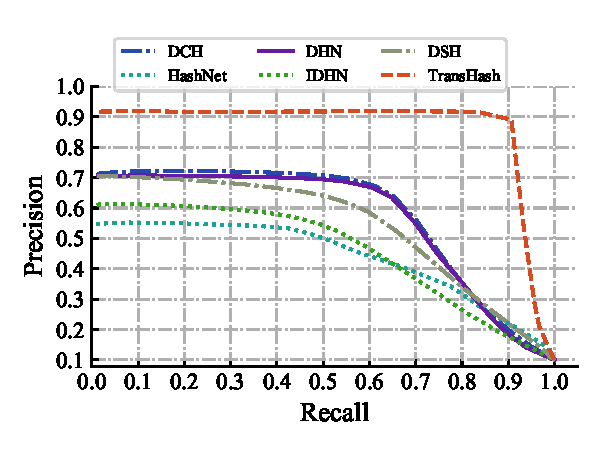
\includegraphics[height=5cm]{04/cifar_16b_pr.pdf}
    \caption{16位哈希码下在\textbf{CIFAR}上各种方法的\textbf{PR}曲线}
  \end{subfigure}
  \hspace{1cm}
  \begin{subfigure}{0.45\textwidth}
    \centering
    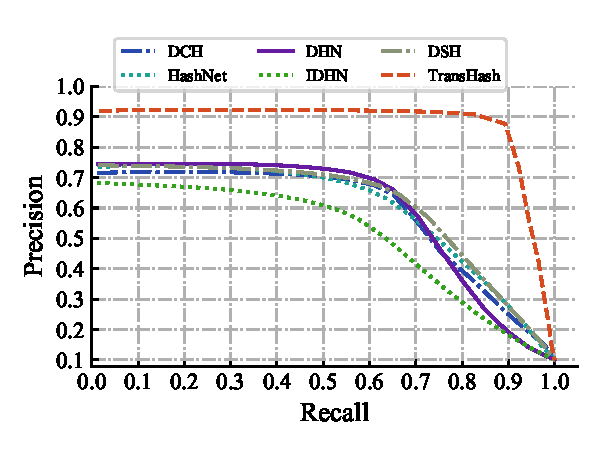
\includegraphics[height=5cm]{04/cifar_64b_pr.pdf}
    \caption{64位哈希码下在\textbf{CIFAR}上各种方法的\textbf{PR}曲线}
  \end{subfigure}
  \hspace{1cm}
  \begin{subfigure}{0.45\textwidth}
    \centering
    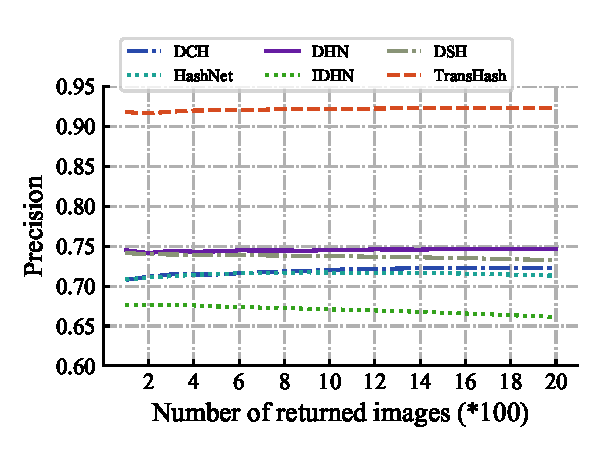
\includegraphics[height=5cm]{04/cifar_48b_topk.pdf}
    \caption{48位哈希码下在\textbf{CIFAR}上各种方法的\textbf{Precision}}
  \end{subfigure}
  \hspace{1cm}
  \begin{subfigure}{0.45\textwidth}
    \centering
    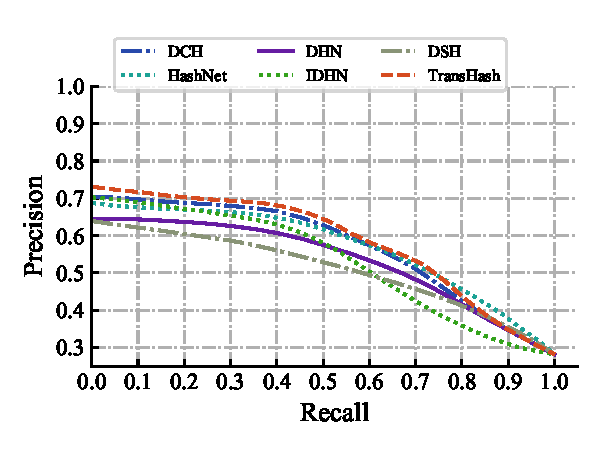
\includegraphics[height=5cm]{04/nuswide_16b_pr.pdf}
    \caption{16位哈希码下在\textbf{NUSWIDE}上各种方法的\textbf{PR}曲线}
  \end{subfigure}
  \hspace{1cm}
  \begin{subfigure}{0.45\textwidth}
    \centering
    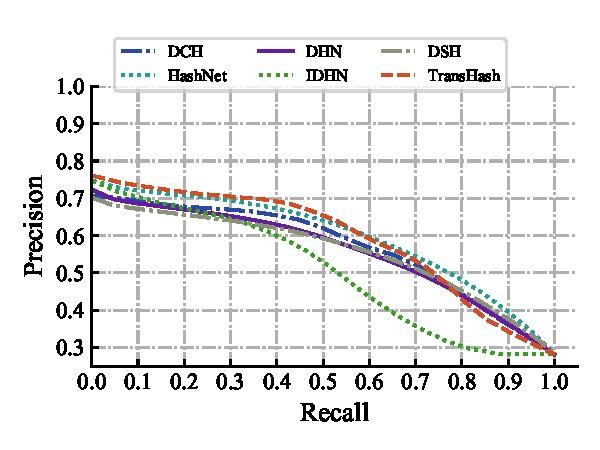
\includegraphics[height=5cm]{04/nuswide_64b_pr.pdf}
    \caption{64位哈希码下在\textbf{NUSWIDE}上各种方法的\textbf{PR}曲线}
  \end{subfigure}
  \hspace{1cm}
  \begin{subfigure}{0.45\textwidth}
    \centering
    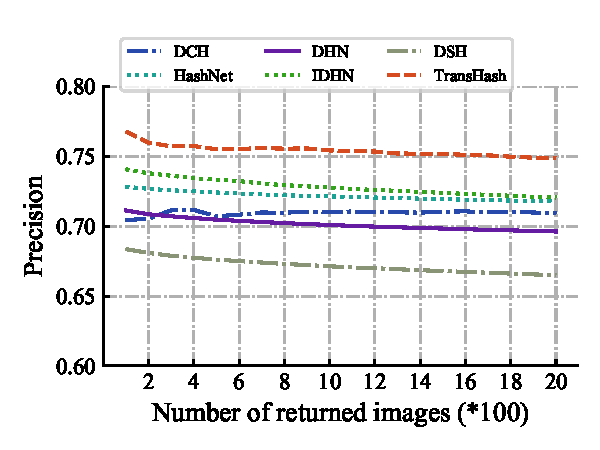
\includegraphics[height=5cm]{04/nuswide_48b_topk.pdf}
    \caption{48位哈希码下在\textbf{NUSWIDE}上各种方法的\textbf{Precision}}
  \end{subfigure}
\end{figure}
\begin{figure}[!htp]\ContinuedFloat
  \hspace{1cm}
  \begin{subfigure}{0.45\textwidth}
    \centering
    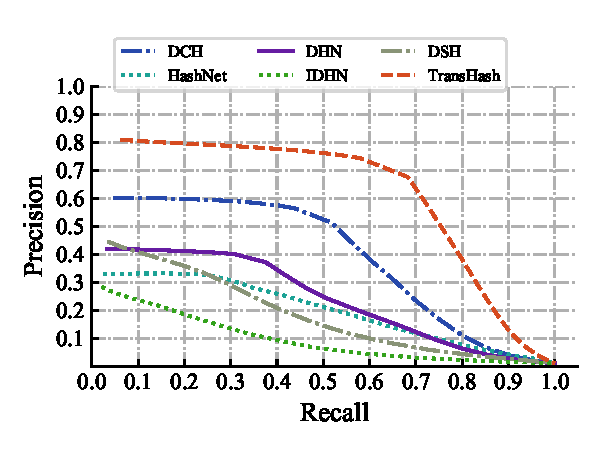
\includegraphics[height=5cm]{04/imagenet_16b_pr.pdf}
    \caption{16位哈希码下在\textbf{IMAGENET}上各种方法的\textbf{PR}曲线}
  \end{subfigure}
  \begin{subfigure}{0.45\textwidth}
    \centering
    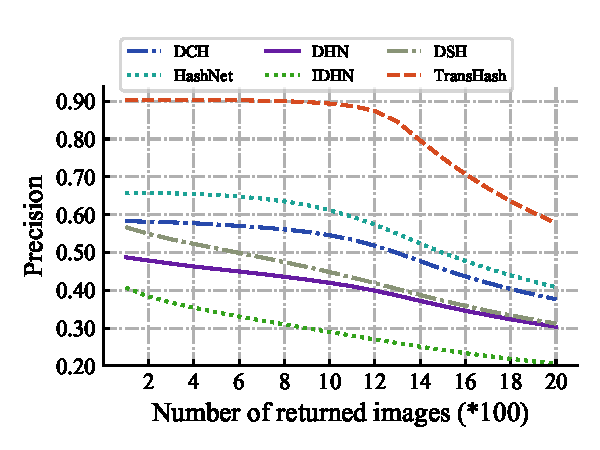
\includegraphics[height=5cm]{04/imagenet_48b_topk.pdf}
    \caption{48位哈希码下在\textbf{IMAGENET}上各种方法的\textbf{Precision}}
  \end{subfigure}
  \bicaption[各种先进哈希算法在三个数据集上的检索结果]{ \textbf{TransHash}和其他算法在不同数据集上的检索结果}{The experimental results on three public benchmark datasets of \textbf{TransHash} and other competing methods.}
  \label{fig:transhashresults}
\end{figure}


我们额外画了基于深度学习的比较模型和\textbf{TransHash}在$16$位哈希码下的\textbf{Precision-Recall}曲线以及在不同的检索返回的图片数量下的\textbf{Precision}曲线。如图~\ref{fig:transhashresults}所示, 对于\textbf{PR}曲线, 代表\textbf{TransHash}的红色曲线始终以大幅度领先其他比较的算法。而对于\textbf{Precision}曲线, \textbf{TransHash}也显著高于所有其他的曲线。在\textbf{NUSWIDE}上, \textbf{TransHash}在\textbf{PR} 曲线上只以微小的优势超过其余方法。对于\textbf{Precision}曲线, \textbf{TransHash}对于检索的返回图片数为$100$时, 得到的精度为$76.77 \%$, 超过\textbf{IDHN}$2.7 \%$。 在\textbf{IMAGENET}, 同样可以观察到非常显著的性能提升。对于$16$位哈希码的\textbf{Precision-Recall}曲线, \textbf{DCH}取得了第二的性能而在$48$时, \textbf{HashNet}则超越了\textbf{DCH}取得了第二的性能。同时很容易观察到\textbf{TransHash}在两种评估指标上都以大幅度领先其余比较的方法。在\textbf{Precision}上, 在检索返回图片数量为$100$和$1000$时候, 我们分别取得$90.35\%$和$ 89.38\%$的精度, 超越\textbf{HashNet} $24.73\%$ 和 $28.18 \%$。这些卓越的性能结果可以充分的证实本章提出的纯粹基于Transformer的深度哈希架构的有效性。


\begin{figure}[!htp]
  \begin{subfigure}{0.45\textwidth}
    \centering
    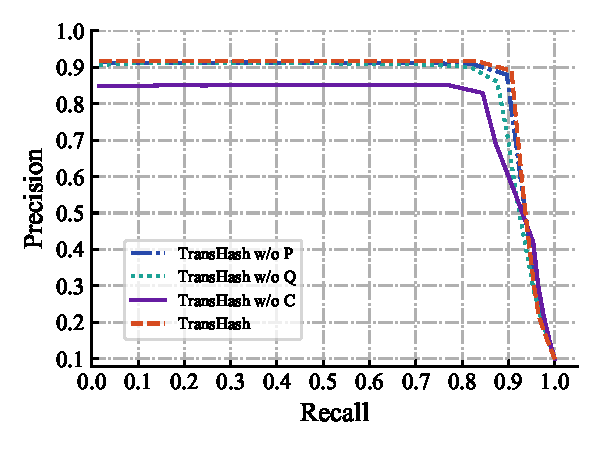
\includegraphics[height=5cm]{04/cifar_16b_ab_pr.pdf}
    \caption{16位哈希码下在\textbf{IMAGENET}上各种方法的\textbf{PR}曲线}
  \end{subfigure}
  \hspace{1cm}
  \begin{subfigure}{0.45\textwidth}
    \centering
    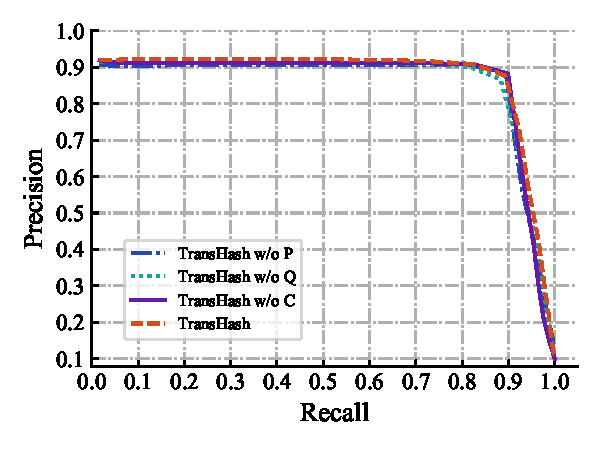
\includegraphics[height=5cm]{04/cifar_64b_ab_pr.pdf}
    \caption{48位哈希码下在\textbf{IMAGENET}上各种方法的\textbf{Precision}}
  \end{subfigure}
  \hspace{1cm}
  \begin{subfigure}{0.45\textwidth}
    \centering
    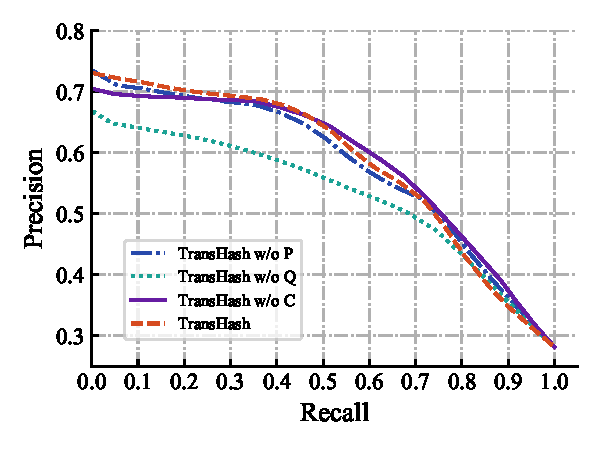
\includegraphics[height=5cm]{04/nuswide_16b_ab_pr.pdf}
    \caption{16位哈希码下在\textbf{IMAGENET}上各种方法的\textbf{PR}曲线}
  \end{subfigure}
  \hspace{1cm}
  \begin{subfigure}{0.45\textwidth}
    \centering
    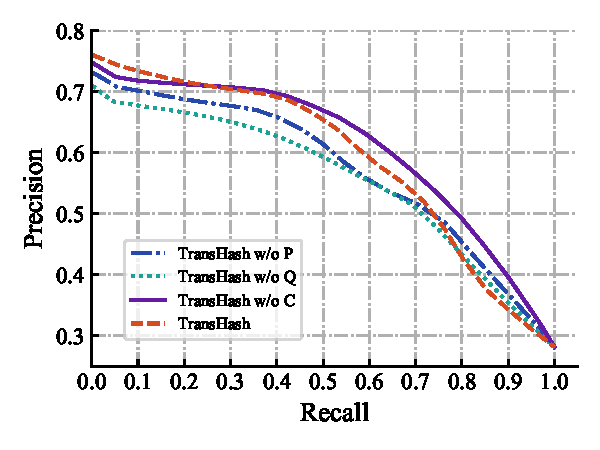
\includegraphics[height=5cm]{04/nuswide_64b_ab_pr.pdf}
    \caption{48位哈希码下在\textbf{IMAGENET}上各种方法的\textbf{Precision}}
  \end{subfigure}
  \hspace{1cm}
  \begin{subfigure}{0.45\textwidth}
    \centering
    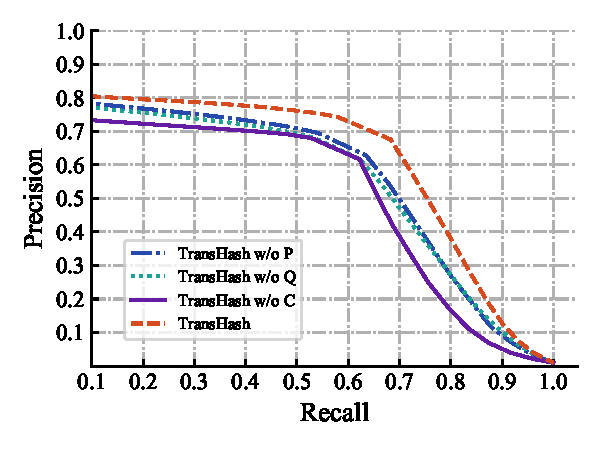
\includegraphics[height=5cm]{04/imagenet_16b_ab_pr.pdf}
    \caption{16位哈希码下在\textbf{IMAGENET}上各种方法的\textbf{PR}曲线}
  \end{subfigure}
  \hspace{1cm}
  \begin{subfigure}{0.45\textwidth}
    \centering
    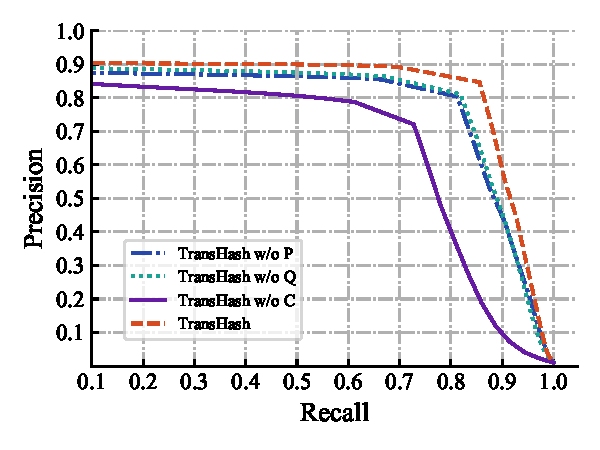
\includegraphics[height=5cm]{04/imagenet_64b_ab_pr.pdf}
    \caption{48位哈希码下在\textbf{IMAGENET}上各种方法的\textbf{Precision}}
  \end{subfigure}
  \bicaption[在三个数据集上的消融实验的结果]{ \textbf{TransHash}和其他变种在三个数据集上的结果}{The experimental results on three public benchmark datasets of \textbf{TransHash} and three variants.}
  \label{fig:ablationresults}
\end{figure}


\subsection{消融实验}
为了进一步分析本章提出的整个算法框架, 我们进行了一个详细的消融实验来证实框架每一个组成部分的有效性。具体而言, 我们研究了三种基于\textbf{TransHash}的变种:
\begin{enumerate}
    \item \textbf{TransHash w/o P:} 是没有双流特征学习机制的\textbf{TransHash}变种。
    \item \textbf{TransHash w/o Q:} 是没有柯西分布的量化损失函数的变种。
    \item \textbf{TransHash w/o C:} 是继续采取\textit{sigmoid}函数作为生成概率的函数$\sigma(.)$的变种。
\end{enumerate}
如表~\ref{table:ablation} 和 图~\ref{fig:ablationresults}所示, 当没有柯西量化损失函数时, 如\textbf{TransHash w/o Q}所示, 框架经受了明显的性能下降。在\textbf{NUSWIDE}和\textbf{IMAGENET}下, $64$位哈希码的情况下\textbf{mAP}分别从 74.88\% 下降到 69.15\% 以及89.21\% 下降到 87.58 \%。当模型没有采取柯西分布作为概率生成函数时, 如\textbf{TransHash w/o C}所示, 我们可以观察点显著的性能下降。具体来说, 在\textbf{IMAGENET}上, 模型经历了平均$5.55 \%$的\textbf{mAP}下降。我们也注意到在哈希码较短的情况下, 模型的性能损失更加显著。主要的原因是根据Cao~\cite{cao2018deep}, 柯西分布可以有效的拉近相似对的哈希距离至一个较小的范围内, 这使得其在哈希码短的情况下更加的明显。\par



最重要的是, 为了测试本章提出的双流特征学习的有效性, 我们也测试了本章提出的孪生模型仅仅包含全局特征学习时时候的性能。如图~\ref{fig:ablationresults}所示,  \textbf{TransHash w/o P} 的性能持续性的低于具有我们提出的双流特征学习机制的完全模型。在\textbf{NUSWIDE} 和 \textbf{IMAGENET}上, 平均的\textbf{mAP}下降分别是  2.08\% 和 2.83\%。这些实验充足的证明了我们提出的纯基于Transformer的框架的各个组成部分的有效性。\par
由于控制本框架的局部特征的数量的超参数$K$对于模型来说也非常的重要, 我们额外在\textbf{CIFAR-10}进行了详细的实验来对$K$值的敏感性进行探讨。值得注意的是, 如果最终的哈希码的长度是$16$, 并且$K$为2时, 则全局的特征负责生成第一个$8$位的哈希码, 而其余的局部特征每一个负责生成$4$位的哈希码。 \par
如表~\ref{table:ablationk}所示, 通常而言, 模型的性能对$K$的取值并不敏感。同时, 我们也注意到, 当每一个局部特征向量对应生成的哈希码长度少于$4$时候, 模型通常不能收敛。鉴于以上的观察, 我们根据经验将$K$的值设置为$2$。

\begin{table}[!htpb]
    %% \centering % not needed
    \bicaption{$K$值的敏感性分析。`-'指的是模型不能收敛 }{Analysis of the effects of K on CIFAR-10. Note that `-' denotes when K equals a certain number, the model fails
    to converge as illustrated in the empirical analysis.}
    \centering
    \begin{tabular}{ccccccc}
       \\ \hline
    
    \multicolumn{2}{l|}{Groups (K)} & 2 & 3 & 4 & 5  & 66 \\\hline
    \hline
    \multicolumn{2}{l|}{\textbf{16 bits}} & 0.9075 & - & - & - & -  \\
    \multicolumn{2}{l|}{\textbf{32 bits}} & 0.9075 & 0.9013 & - & - & -  \\
    \multicolumn{2}{l|}{\textbf{48 bits}} & 0.9141 & 0.9017 & 0.9187 & 0.9107 & 0.9143 \\
    \multicolumn{2}{l|}{\textbf{64 bits}} & 0.9166 & 0.9103 & 0.9057 & 0.9062 & 0.8994  \\
    \hline 
    \hline
    \end{tabular}
    \label{table:ablationk}
  \end{table}


\section{总结}
在本章中, 我们提出了一个完全基于Transformer的深度哈希框架-\textbf{TransHash}来解决具有挑战性的大规模图像检索的问题。具体来说, 我们提出了一个新型的基于孪生Vision Transformer的架构基于成对的相似度矩阵来提取强健的有判别力的特征。同时, 我们提出设计一个双流特征学习机制来同时学习全局和局部的特征, 从而得到更加细粒度的特征表示。为了进行相似度保留学习, 本章基于一个带权重的贝叶斯学习框架来进行度量学习。本章提出的框架可以通过一个端到端的学习方法进行训练优化。我们在三个标准的大规模图像检索数据集上进行了训练和测试。实验结果表明我们的模型在\textbf{CIFAR-10},~\textbf{NUSWIDE}和~\textbf{IMAGENET}上, 相比较其他先进的基于卷积神经网络的算法可以获得显著的性能提升。